% Pre-ambulo
\documentclass[a4paper, 12pt]{abnt}

\usepackage{ucs}
\usepackage[brazil]{babel}
\usepackage[utf8]{inputenc}
\usepackage[T1]{fontenc}
\usepackage{dsfont}
\usepackage{amssymb,amsmath}
\usepackage{multirow}
\usepackage[pdftex, colorlinks=true, citecolor=blue, urlcolor=blue, linkcolor=black]{hyperref}
\usepackage[num, no-abnt-option-file]{abntcite}
\usepackage[pdftex]{color, graphicx}
\usepackage{colortbl}
\usepackage{url}
\usepackage{abnt-num}
\usepackage{abntcite}
\usepackage{algorithm}
\usepackage{algorithmic}
\usepackage{etoolbox}
\usepackage{enumerate}
\usepackage{rotating}
\usepackage[section]{placeins}
\usepackage{pdflscape}
\usepackage{longtable}
\usepackage[final]{pdfpages}

\usepackage[proportional,scaled=1.064]{erewhon}
\renewcommand*\oldstylenums[1]{\textosf{#1}}

\setcounter{secnumdepth}{5}

%\usepackage{alg}

\citebrackets[]

% Redefinicao de instrucoes
\floatname{algorithm}{Algoritmo}
\renewcommand{\algorithmicrequire}{\textbf{Entrada:}}
\renewcommand{\algorithmicensure}{\textbf{Saída:}}
\renewcommand{\algorithmicend}{\textbf{fim}}
\renewcommand{\algorithmicif}{\textbf{se}}
\renewcommand{\algorithmicthen}{\textbf{então}}
\renewcommand{\algorithmicelse}{\textbf{senão}}
\renewcommand{\algorithmicfor}{\textbf{para}}
\renewcommand{\algorithmicforall}{\textbf{para todo}}
\renewcommand{\algorithmicdo}{\textbf{faça}}
\renewcommand{\algorithmicwhile}{\textbf{enquanto}}
\renewcommand{\algorithmicloop}{\textbf{loop}}
\renewcommand{\algorithmicrepeat}{\textbf{repetir}}
\renewcommand{\algorithmicuntil}{\textbf{até que}}
\renewcommand{\algorithmiccomment}[1]{\% #1}

\renewcommand{\author}{Adorilson Bezerra de Araújo}
\newcommand{\mscThesisTitle}{Estudo Empírico de Análise da Compatibilidade de
Aplicações Android com Diferentes Versões da API da Plataforma}
\newcommand{\mscThesisEnglishTitle}{Empirical Study of Analysis on Android Application
Compatibility with Different Versions of the Platform API}
\newcommand{\advisor}{Prof. Dr. Uirá Kulesza}

\newif\ifcoadvisor
\coadvisorfalse
\newcommand{\coadvisor}{}

\newcommand{\city}{Natal-RN}
\renewcommand{\date}{Fevereiro de 2017}

% Definicao da lista de simbolos
% \simb[entrada na lista de simbolos]{simbolo}:
% Escreve o simbolo no texto e uma entrada na lista de simbolos.
% Se o parametro opcional e omitido, usa-se o parametro obrigatorio.
\newcommand{\simb}[2][]
{%
	\ifthenelse{\equal{#1}{}}
	{\addcontentsline{los}{simbolo}{#2}}
	{\addcontentsline{los}{simbolo}{#1}}#2
}
% Para aceitar comandos com @ (at) no nome
\makeatletter 
% \listadesimbolos: comando que imprime a lista de simbolos
\newcommand{\listadesimbolos}
{
	\pretextualchapter{Lista de símbolos}
	{\setlength{\parindent}{0cm}
	\@starttoc{los}}
}
% Como a entrada sera impressa
\newcommand\l@simbolo[2]{\par #1}
\makeatother


% Definicao da lista de abreviaturas e siglas
% \abrv[entrada na lista de simbolos]{abreviatura}:
% Escreve a sigla/abreviatura no texto e uma entrada na lista de abreviaturas e siglas.
% Se o parametro opcional e omitido, usa-se o parametro obrigatorio.
\newcommand{\abrv}[2][]
{%
	\ifthenelse{\equal{#1}{}}
	{\addcontentsline{loab}{abreviatura}{#2}}
	{\addcontentsline{loab}{abreviatura}{#1}}#2
}
% Para aceitar comandos com @ (at) no nome
\makeatletter 
% \listadeabreviaturas: comando que imprime a lista de abreviaturas e siglas
\newcommand{\listadeabreviaturas}
{
	\pretextualchapter{Lista de abreviaturas e siglas}
	{\setlength{\parindent}{0cm}
	\@starttoc{loab}}
}
% Como a entrada sera impressa
\newcommand\l@abreviatura[2]{\par #1}
\makeatother

\makeatletter
\renewcommand\@biblabel[1]{[#1] \hspace{5 mm}}
\apptocmd{\thebibliography}{\setlength\itemindent{-30pt}}{}{}
\makeatother


% \listofalgorithms: comando que imprime a lista de algoritmos
\renewcommand{\listalgorithmname}{Lista de algoritmos}


% Hifenização de palavras feita de forma incorreta pelo LaTeX
\hyphenation{PYTHON ou-tros}


% Inicio do documento
\begin{document}

	\frenchspacing
	
	% Capa (arquivo Includes/Capa.tex)
	% Capa
% Proteção externa do trabalho e sobre a qual se imprimem as informações indispensáveis 
% à sua identificação.

% Especificação da capa
\begin{titlepage}
	\begin{center}
		
		% Cabeçalho (não deve ser modificado)
		% Contém o brasão da Universidade, o logotipo do Departamento, além dos dados
		% relacionados à vinculação do aluno (Universidade, Centro, Departamento e Curso)
		\begin{minipage}{15.15cm}
			\begin{center}
				
\includegraphics[width=2.25cm, height=2.68cm]{imagens/logo}
				\begin{espacosimples}
					{\small \ \\
                       \textsc{Universidade Federal do Rio Grande do Norte}		   			\\
							  \textsc{Centro de Ciências Exatas e da Terra}					\\
							  \textsc{Programa de Pós-Graduação em Sistemas e Computação}  	\\
                       \textsc{Mestrado Acadêmico em Sistemas e Computação}}   				\\
				\end{espacosimples}
			\end{center}
		\end{minipage}
		
			
		\vspace{5cm}
						
		% Tíulo do trabalho
		{\setlength{\baselineskip}%
		{1.3\baselineskip}
		{\LARGE \textbf{\mscThesisTitle}}\par}
			
		\vspace{3cm}
			
		% Nome do aluno (autor)
		{\large \textbf{\author}}
						
		\vspace{5cm}
		
		% Local da instituição onde o trabalho deve ser apresentado e ano de entrega do mesmo
		{\city} \\ {\date}
	\end{center}
\end{titlepage}

	% Folha de rosto (arquivo Includes/FolhaRosto.tex)
	% Folha de rosto
% Contém os elementos essenciais à identificação do trabalho.

% Título, nome do aluno e respectivo orientador e filiação
\titulo{\Large{\mscThesisTitle}}
\autor{\author}
\orientador[Orientador]{\par \advisor}

\ifcoadvisor
\coorientador[Coorientador]{\par \coadvisor}
\fi

\instituicao
{
	PPgSC -- Programa de Pós-Graduação em Sistemas e Computação\par 
   CCET -- Centro de Ciências Exatas e da Terra\par
   UFRN -- Universidade Federal do Rio Grande do Norte
}
	
% Natureza do trabalho (não deve ser modificada)
\comentario
{
	Dissertação de Mestrado apresentada ao Programa de Pós-Graduação em Sistemas e Computação, do Centro de Ciências Exatas e da Terra, da Universidade Federal do Rio Grande do Norte como requisito parcial para a obtenção do grau de Mestre em Sistemas e Computação.\bigskip\\
   \textit{Linha de pesquisa}:\\Engenharia de Software
}
		
% Local e data
\local{\city}
\data{\date}
	
\folhaderosto
	
	
	% Folha de aprovacao (arquivo Includes/FolhaAprovacao.tex)
	% Folha de aprovação
\begin{folhadeaprovacao}

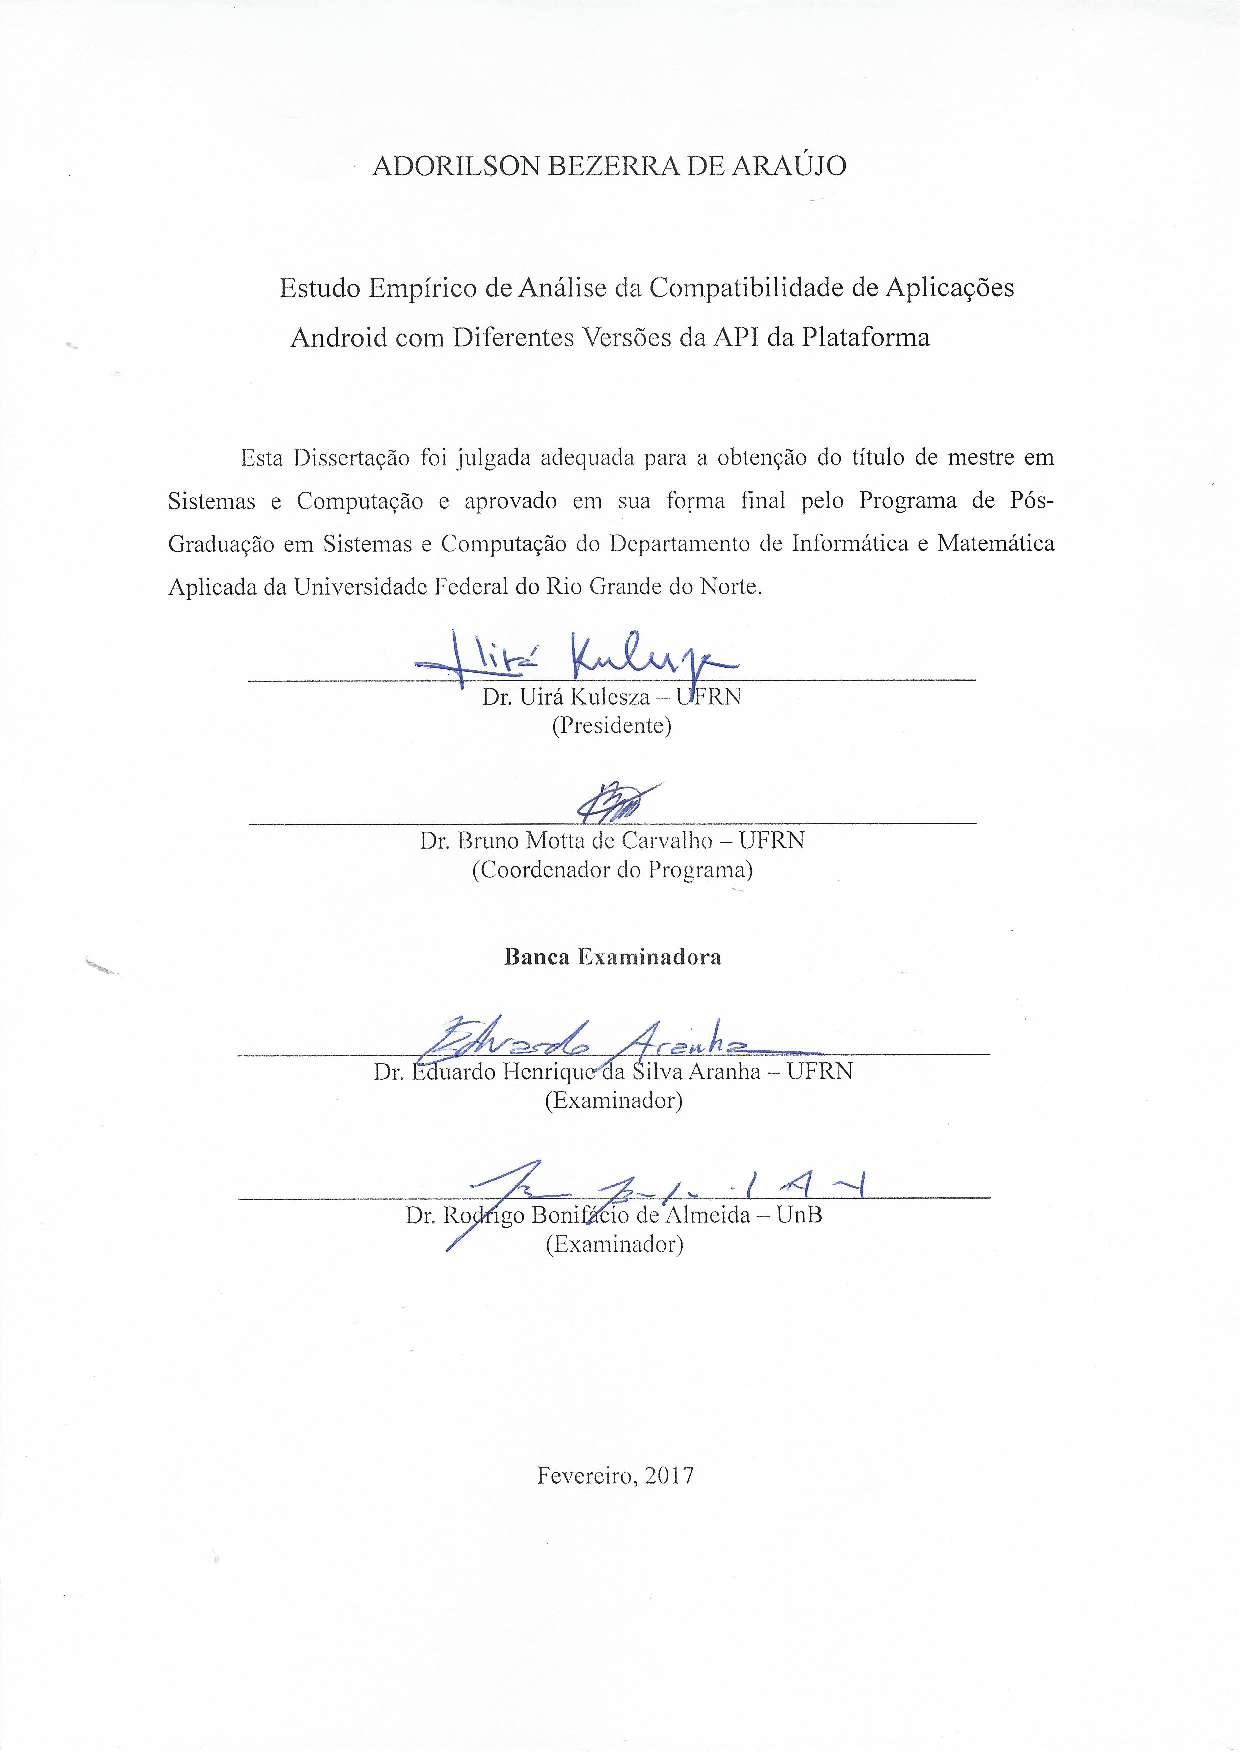
\includepdf[pages=-]{Includes/folha_aprovacao.pdf}
	
\end{folhadeaprovacao}	
	
	% Dedicatoria (arquivo Includes/Dedicatoria.tex)
	%% Dedicatória

\chapter*{}
\vspace{15cm}
\begin{flushright}
	Homenagem que o autor presta a uma ou mais pessoas.
\end{flushright}
	
	% Agradecimentos (arquivo Includes/Agradecimentos.tex)
	%% Agradecimentos

\chapter*{Agradecimentos}

Agradecimentos dirigidos àqueles que contribuíram de maneira relevante à elaboração do trabalho, sejam eles pessoas ou mesmo organizações.
   
   % Epigrafe (arquivo Includes/Epigrafe.tex)
	%% Epírafe (citação seguida de indicação de autoria)

\chapter*{}
\vspace{15cm}
\begin{flushright}
	\textit
	{
		Citação
	}\medskip\\ 
	Autor
\end{flushright}
	
	% Resumo em língua vernacula (arquivo Includes/Resumo.tex)
	% Resumo em língua vernácula
\begin{center}
	{\Large{\textbf{\mscThesisTitle}}}
\end{center}

\vspace{1cm}

\begin{flushright}
	Autor: \author\\
	Orientador(a): \advisor \\
	
	\ifcoadvisor
	Coorientador(a): \coadvisor
	\fi
	
	 
\end{flushright}

\vspace{1cm}

\begin{center}
	\Large{\textsc{\textbf{Resumo}}}
\end{center}

\noindent Dispositivos móveis estão ficando cada vez mais populares e acessíveis para pessoas
de diferentes poder aquisitivo ao redor do mundo. A plataforma Android é atualmente
a mais popular para o desenvolvimento de aplicações móveis, ocupando mais de 80\%
do mercado de sistemas operacionais para aplicações de dispositivos móveis. Tal
realidade cria uma demanda por customizações de aplicações para lidar com diferentes
dispositivos, tais como tamanho de tela disponibilidade de poder de processamento
e memória disponível, idiomas e necessidades específicas dos usuários. Além disso,
a bibliotecas de classes da plataforma (API - Application Programming Interface)
evolui muito rapidamente. Já foram disponibilizadas 23 versões desde o lançamento. 
Portanto, é fundamental para o sucesso das aplicações o suporte a múltiplas versões
da API. Apesar da popularidade e ampla gama de aplicações Android já desenvolvida,
existe uma carência de estudos que investiguem a forma como aplicações Android lidam
com essa variabilidade.

\noindent Esta dissertação de mestrado tem como objetivo principal analisar, caracterizar e
comparar técnicas utilizadas por aplicações Android para suporte a múltiplas versões
da API. Em especial, o trabalho busca:
(i) Identificar na literatura quais as técnicas indicadas para suporte a múltiplas versões da API Android;
(ii) Analisar aplicações reais para quantificar o uso dessas técnicas indicadas; e
(ii) Comparar as características e consequências do uso de tais técnicas.

\noindent\textit{Palavras-chave}: gerência de variabilidades, implementação de variabilidades, aplicações
Android, plataforma de computação móvel, estudos empíricos, suporte multi-versão de API

	
	% Abstract, resumo em língua estrangeira (arquivo Include/Abstract.tex)
	% Resumo em língua estrangeira (em inglês Abstract, em espanhol Resumen, em francês Résumé
\begin{center}
	{\Large{\textbf{\mscThesisEnglishTitle}}}
\end{center}

\vspace{1cm}

\begin{flushright}
	Author: \author\\
	Advisor: \advisor \\
	Co-advisor: \coadvisor
\end{flushright}

\vspace{1cm}

\begin{center}
	\Large{\textsc{\textbf{Abstract}}}
\end{center}

\noindent Applications are increasingly inserted into society through various devices. Many of them are complex due to their scale, making their architecture also complex to understand and maintain. The software visualization area uses techniques that aim to improve software understanding and make its development process more productive. The lack of activities for developers and architects to understand the architectural evolution can lead to its degradation, causing the quality criteria initially set no longer met. In this sense, in relation to measuring the performance of applications, profiling tools and APM can be used, however, fail to provide adequate metrics and visualizations to monitor the evolution of this quality attribute. This work presents a set of software visualizations to help analyze the evolution of performance between versions of a software, allowing developers and architects to identify methods of scenarios that have degraded or improved their performance. The proposed set of visualizations will be evaluated from empirical studies conducted in open source applications.

\noindent\textit{Keywords}: software architecture, software visualization, software evolution.
	
	% Lista de figuras
	\listoffigures

	% Lista de tabelas
	\listoftables
	
	% Lista de abreviaturas e siglas
	\listadeabreviaturas
	
	% Lista de símbolos
	%\listadesimbolos
	
	% Lista de algoritmos (se houver)
	% Devem ser incluídos os pacotes algorithm e algorithmic
	% \listofalgorithms
	
	% Sumário
	\sumario

	% Parte central do trabalho, englobando os capítulos que constituem o mesmo
	% Os referidos capítulos devem ser organizados dentro do diretório "Capítulos"

	% Capitulo 1: Introdução (arquivo Includes/Introducao.tex)
	% Introdução
\chapter{Introdução} \label{ch:introducao}

Dispositivos móveis estão ficando cada vez mais populares e acessíveis para
pessoas de diferentes poder aquisitivo ao redor do mundo \cite{Lhamas2014}.
A plataforma Android é atualmente a mais popular para o desenvolvimento de
aplicações móveis, ocupando mais de 80\% do mercado de sistemas operacionais
para aplicações de dispositivos móveis \cite{jim2014}. Tal realidade cria uma
demanda por customizações de aplicações para lidar com diferentes dispositivos,
tais como, tamanho de tela, bibliotecas de classes disponíveis 
\abrv[API -- \textit{Application Programming Interface}]
{(API - \textit{Application Programming Interface}),} % esse virgula dentro do {}
													  % é grambiarra por causa de um
													  % espaço gerado após o }
disponibilidade de poder de processamento e memória, idiomas e
necessidades específicas dos usuários. O Facebook, por exemplo, disponibiliza
duas versões do seu aplicativo. A versão padrão é direcionada para os dispositivos
mais modernos e a alternativa, chamada de Facebook Lite\footnote{Disponível em:
https://play.google.com/store/apps/details?id=com.facebook.lite},
para dispositivos mais antigos (que utilizam a partir da versão 2.2 do Android),
que ocupa bem menos espaço de armazenamento, pode ser carregada na memória do
dispositivo mais rapidamente e funciona com conexões de Internet instáveis ou lentas.

A existência de diferentes dispositivos para os quais a plataforma Android oferece
suporte é conhecido como fragmentação, e isso se apresenta como um grande desafio
em relação à outras plataformas. Há um número considerável de dispositivos com versões
antigas da API \cite{Gronli2014}. Já em 2011, 86\% dos desenvolvedores consideravam
a fragmentação da plataforma um sério problema \cite{Elmer-DeWitt2011}.
Diferentes versões da API é uma das variabilidades mais comuns na plataforma Android.
Esse cenário leva os desenvolvedores de aplicações Android a buscarem técnicas e
metodologias que otimizem o desenvolvimento de versões da aplicação que melhor
atendam às restrições e características de cada dispositivo. A documentação oficial
do Android \cite{GuiaAndroid} é rica em propor soluções para tais variabilidades,
no entanto, a implementação dessas soluções pode sofrer variações. Cada equipe
de desenvolvimento pode tomar decisões de projeto diferentes. Em especial, existe
atualmente uma carência de estudos sobre a forma como aplicações Android atuais
oferecem suporte às múltiplas versões da API. Neste contexto, este trabalho busca
entender as técnicas utilizadas para oferecer tal suporte e qual o impacto do seu uso.

\section{Problema Abordado} \label{sec:apresentacao-do-problema}

Apesar da ampla adoção da plataforma Android e o problema da fragmentação \cite{Park2013},
há uma carência de estudos que indiquem de que forma as aplicações de tal plataforma
lidam e se adaptam às diversas versões lançadas da API. 
Enquanto atender a usuários com uma antiga versão da API significa ter um amplo
mercado potencial, utilizar os recursos das versões mais novas da API é um dos três 
fatores mais importantes para as aplicações com alta avaliação na Google Play \cite{Tian2015}.
Oferecer suporte a múltiplas versões da API da plataforma, de forma a atender clientes
com versões antigas ao mesmo tempo usar os recursos mais modernos quando disponíveis,
é primordial para o sucesso das aplicações.

Uma alternativa possível é disponibilizar uma versão da aplicação para cada versão
da API. Essa solução é a comumente utilizada para API’s locais - API’s de sistemas
operacionais de computadores de mesa, por exemplo -, onde o número de versões de
API’s é reduzido e a evolução é mais lenta em comparação à API do Android, na qual
existem
cerca de 10 versões da API com uma margem relevante do mercado. Manter diversas
versões simultâneas de uma aplicação causa duplicação de código e prejudica a
manutenibilidade. % TODO colocar referencia aqui
Assim, a plataforma oferece mecanismos para que uma única base
de código atenda da melhor forma possível às diversas versões da API, usando os
melhores recursos disponíveis nos aparelhos.

No entanto, no melhor do nosso conhecimento, não existem estudos sistemáticos que
identifiquem e analisem técnicas para implementação de suporte às
múltiplas versões da plataforma Android. Tais estudos podem trazer luz sobre as
práticas adotadas pela comunidade de desenvolvedores e auxiliá-los a decidir
quando e quais técnicas melhor atendem a determinadas situações.

\section{Limitações de Trabalhos Existentes} \label{sec:limitacao-abordagens-atuais}
Diversos trabalhos têm sido realizados sobre a API da plataforma Android. Sobretudo,
no sentido
de identificar os elementos mais comuns e padrões de uso. Lamba et al.\cite{Lamba2015} apresentaram
resultados de um estudo em larga escala de análise do uso da API em aplicações Android.
O estudo envolveu 1.120 aplicações open-source e 17,4 milhões de linha de código.
Foram identificados os métodos mais frequentemente invocados, os pacotes da API,
classes, e padrões de chamadas mais populares.Os métodos mais comuns são \texttt{getString()},
\texttt{get()} e \texttt{toString()}. Os pacotes mais comuns são \texttt{java.util} e
\texttt{android.content}. As classes mais comuns são \texttt{Context} e \texttt{View}.
O padrão de chamada mais popular está relacionado à dimensão, espaçamento e margens
de uma \textit{view} na interface com o usuário. No entanto, na análise de popularidade
de métodos não levaram em consideração suas respectivas classes. Por exemplo, o método
\texttt{getString()} da classe \texttt{Activity} foi contabilizado juntamente com
o método \texttt{getString()} da classe \texttt{Cursor}, que não possuem nenhuma
relação entre si.

McDonnell et al. \cite{McDonnell2013} conduziram um estudo sobre a co-evolução
da API Android e suas aplicações usando o histórico de versões encontradas no
Github. O estudo confirmou que a plataforma Android evolui rapidamente em uma
taxa de 115 mudanças da API por mês na média. Contudo, a adoção pelas aplicações
clientes não segue na mesma velocidade. Cerca de 28\% das referências à API nas
aplicações clientes estão desatualizadas com uma mediana de tempo de 16 meses.
22\% das referências desatualizadas são eventualmente atualizadas para versões
mais novas da API, mas com um tempo de propagação de cerca de 14 meses, que é mais
lento que o tempo médio entre novas versões da API (3 meses). API's de rápida
evolução são mais usadas por clientes que APIs de evolução lenta, mas o tempo
médio necessário para adoção de novas versões é mais longo para APIs de rápida
evolução. Além disso, código adaptado para uso de novas APIs são mais sujeitos a
erros que aqueles sem adaptação para novas APIs. Segundo os autores do trabalho,
os resultados sugerem que os desenvolvedores não adotam novas API's com rapidez,
mantendo referências para API's desatualizadas. Assim evitam a instabilidade de
novas API's e o trabalho de atualização propriamente dito. Porém, outras possibilidades
devem ser consideradas: os desenvolvedores atualizam para as mais recentes API's,
mas mantém tais códigos para garantir a compatibilidade com API's mais antigas;
ou atualizam para API's recentes e as referências às API's antigas representam
código-morto.

Aplicações Android declaram uma versão alvo da API. Quando estão em execução em
um dispositivo cuja versão da API é inferior à versão alvo, as aplicações são
executadas em um modo de compatibilidade, que busca reproduzir o comportamento
da versão alvo indicada pelo aplicação. Esse cenário desabilita as melhorias da
nova versão, incluindo as correções de problemas de segurança. Mutchler et al.
\cite{Mutchler2016}
chamam essa característica de problema da fragmentação do alvo e analisam um
conjunto de 1.232.696 aplicações Android para mostrar que isso traz sérias
consequências para todo o ecossistema de aplicações e não mudou consideravelmente
com o 
passar dos anos. No total, 93\% das aplicações atualmente definem como alvo uma
versão desatualizada e possuem uma média de desatualização de 686 dias; 79\% das
aplicações já estão desatualizadas no dia que são carregadas para o Google Play.
Eles também analisaram 5 mudanças na plataforma relacionadas a segurança e que estão
desabilitadas nessas aplicações desatualizadas.

Wei \cite{Wei2016} realizou um estudo sobre problemas de compatibilidade induzidos
pela fragmentação 
\abrv[FIC -- \textit{Fragmentation-Induced Compatibility}]
(FIC issues - \textit{Fragmentation-Induced Compatibility issues}) da plataforma
Android.
De forma manual, analisaram 191 \textit{issues} nos sistemas de reporte de erros
de 5 projetos de código aberto e os \textit{commits} relacionadas a esses \textit{issues}.
Nesse estudo, identificaram que existem 5 maiores causas de FIC issues, entre elas
a evolução da API. FIC \textit{issues} podem causar tanto consequências funcionais como
não-funcionais, como travamento da aplicação, aplicação não funcionar, degradação
na performance e na experiência de uso. Os sintomas podem ser específicos da aplicação,
o que dificulta a criação de testes de compatibilidade. Localizar a causa dos FIC
\textit{issues} é difícil na prática. Por outro lado, as correções são usualmente
simples e apresentam padrões comuns: checar informações do dispositivo e disponibilidade
de componentes de software/hardware antes de chamar API's/métodos causadores de
problemas. Este é o padrão mais comum, presente em 137 das 191 correções analisadas.
Uma forma típica de evitar os erros é pular a chamada da API ou substituí-la por
uma implementação alternativa. Também desenvolveram uma ferramenta, FicFinder, que
realiza uma análise estática nas aplicações e informa se estas contém FIC
\textit{issues}. Em um experimento com 27 aplicações do mundo real, o FicFinder
efetivamente detectou FIC issues desconhecidos com
uma alta precisão na análise. Nas 27 aplicações foram emitidos 51 alertas, sendo
46 de casos confirmados (precisão de 90,2\%). FicFinder também pode fornecer
informações úteis para ajudar desenvolvedores a diagnosticar e corrigir FIC
\textit{issues}. Os alertas emitidos pelo FicFinder foram encaminhados para os
desenvolvedores das aplicações. Alguns já haviam corrigido o problema e outros
informaram que iriam corrigir.

McDonnell et al. \cite{McDonnell2013} e Mutchler et al. \cite{Mutchler2016}
não abordam o tema de suporte a múltiplas versões da API
por aplicações Android existentes. Todas as análises dos estudos foram
realizadas sem considerar questões como a adaptação e organização do código para
lidar com as múltiplas API's disponíveis.

No experimento realizado por Wei et al. \cite{Wei2016}, o FicFinder foi
alterado para reportar situações em que os FIC \textit{issues} já estavam protegidos
de execuções indevidas, tais casos foram identificados como "boas práticas". Porém,
o trabalho não apresentou essas boas práticas, tampouco fez qualquer tipo de
comparação, avaliação ou indicação de uso.

Nesse contexto, baseado em trabalhos anteriores acerca da evolução da API Android
e suas limitações, são necessárias pesquisas que:
\begin{itemize}
    \item Identifiquem o suporte a múltiplas versão da API provida pela plataforma;
    \item Analisem como tais técnicas são implementadas em aplicações do mundo
        real, de forma qualitativa e quantitativa;
    \item Analisem o impacto do uso de tais técnicas no código-fonte das aplicações
        cliente.   
\end{itemize}

\section{Objetivos} \label{sec:objetivos-gerais-especificos}

O objetivo geral desta dissertação de mestrado é analisar, caracterizar e comparar
técnicas de implementação de suporte a múltiplas versões da API da plataforma
Android por aplicações existentes. Os objetivos específicos do trabalho são:
\begin{itemize}
	\item Identificar na literatura quais as técnicas indicadas para oferecer suporte
	a múltiplas versões da API Android;
	\item Analisar aplicações reais para quantificar o uso dessas técnicas indicadas;
	\item Comparar as características e consequências do uso de tais técnicas; e
	\item Identificar as mudanças mais comuns na API que afeta a evolução das
	aplicações para rodar em aparelhos com versões diferentes da API.
\end{itemize}

\section{Metodologia} \label{sec:metodologia}

Visando atingir os objetivos desta dissertação de mestrado, foi definido uma
metodologia de trabalho composta das seguintes etapas:
\begin{itemize}
	\item Revisão da literatura: essa etapa buscou identificar quais as técnicas
	indicadas pela literatura para oferecer suporte a múltiplas versões da API,
	além de entender melhor os trabalhos relacionados atuais;
	\item Estudo empírico: a partir dos resultados da fase anterior, foi realizado
	um estudo empírico com o objetivo de identificar e caracterizar a adoção dessas
	técnicas por aplicações reais. Ele foi composto das seguintes atividades principais:
	seleção das aplicações, análise das aplicaçõesa e análise dos resultados.
\end{itemize}


\section{Organização do Documento} \label{sec:organizacao-trabalho}

O restante deste documento está organizado da seguinte forma:
\begin{itemize}
    \item O capítulo \ref{ch:fundamentacao-teorica} apresenta os principais
    referenciais teóricos que serviram de arcabouço para o desenvolvimento
    deste trabalho;
    \item O capítulo \ref{ch:estudo}  traz o estudo sobre a compatibilidade
    de aplicações Android com as diferentes versões da API da plataforma. São
    apresentados resultados do estudo e discussão de tais resultados;
    \item No capítulo \ref{ch:trabalhos-relacionados} são discutidos trabalhos
    relacionados;
    \item Por fim, o capítulo \ref{ch:conclusao} apresenta as considerações finais,
    principais contribuições e limitações do trabalho, bem como trabalhos futuros
    de pesquisa que podem ser desenvolvidos como continuidade desta dissertação.
\end{itemize}

	
	% Capitulo 2: Segundo capítulo (arquivo Includes/Capitulo2.tex)
	% Capítulo 2
\chapter{Fundamentação Teórica} \label{ch:fundamentacao-teorica}

Este capítulo apresenta conceitos importantes para a compreensão deste trabalho. A seção \ref{sec:arquitetura-software} explora os conceitos de arquitetura de software e atributos de qualidade, incluindo a definição de cenários. A seção \ref{sec:visualizacao-software} discorre sobre os conceitos de visualização de software, além de definições sobre a visualização da evolução de arquitetura de software. Na seção \ref{sec:ferramentas-analise-desempenho}, são explanados os conceitos empregados nas ferramentas de análise de desempenho. Por fim, na seção \ref{sec:consideracoes-cap2} são apresentadas as considerações finais do capítulo.

\section{Arquitetura de Software} \label{sec:arquitetura-software}

O estudo da arquitetura de software é o estudo de como sistemas de software são projetados e construídos. Ela deve ser o coração do projeto e desenvolvimento de um sistema, estando acima dos processos, análises e do desenvolvimento \cite{Taylor2009}.

A arquitetura de software pode ser definida como a estrutura ou estruturas do sistema, que compreendem os elementos de software, as propriedades externamente visíveis desses elementos e as relações entre eles \cite{Bass2007}. Adicionalmente, de acordo com \citeauthor{Taylor2009}, a arquitetura de um software incorpora todas as decisões de projeto tomadas pelos seus arquitetos, que podem afetar muitos dos seus módulos, incluindo sua estrutura e atributos de qualidade.

Antes da implementação do sistema, decisões arquiteturais tais como quais componentes pertencem a arquitetura do software, quais serviços ou propriedades desses componentes serão externamente visíveis e como eles estão relacionados uns com os outros, devem ser tomadas e deveriam permanecer atendidas durante todo o ciclo de vida do sistema. É igualmente importante o fato de  perceber que a arquitetura do software é essencial para o sistema alcançar os requisitos relacionados aos atributos de qualidade \cite{Kazman2001}.

\subsection{Atributos de Qualidade} \label{subsec:atributos-qualidade}

A medida que o domínio de um software evolui, assim como os seus requisitos, a arquitetura do software precisa ser reavaliada de modo que ainda reflita um sistema moderno que se encaixa no domínio evoluído. Uma arquitetura não é regida apenas por requisitos funcionais, mas em grande parte por atributos de qualidade. Desse modo, criar uma arquitetura apropriada não é uma tarefa trivial \cite{Svahnberg2002}.

A qualidade não pode ser adicionada ao sistema de maneira tardia, pelo contrário, deve ser incorporada desde o início \cite{Svahnberg2002}. Portanto, a arquitetura de um software necessita ser reavaliada para verificar a conformidade dos requisitos funcionais e atributos de qualidade.

Os atributos de qualidade que serão analisados em um processo de avaliação dependem do contexto e domínio do sistema. Uma estratégia comum é abordar os atributos de qualidade mais críticos. Alguns desses atributos são definidos adiante \cite{Kazman2001}:
\begin{itemize}
	\item \textit{Desempenho}: trata da capacidade de resposta do sistema, o tempo requerido para responder a eventos ou o número de eventos processados em determinado intervalo de tempo;
	\item \textit{Confiabilidade}: é a habilidade do sistema se manter operante com o passar do tempo. É geralmente medido pelo tempo médio até a falha;
	\item \textit{Segurança}: mede a habilidade do sistema de resistir a tentativas de uso não autorizado e negação de serviço, enquanto continua fornecendo seus serviços a usuários autorizados;
	\item \textit{Portabilidade}: é a capacidade do sistema de executar em diversos ambientes computacionais.
\end{itemize}

Embora existam outros atributos de qualidade, o atributo de interesse deste trabalho é o desempenho, em termos de tempo de execução. Para medir o desempenho, além do tempo de execução, outras propriedades podem ser usadas, como: consumo de memória, entrada e saída de disco, uso do processador e tráfego de rede \cite{Malik2013}. A medição desse atributo em termos de tempo de execução foi escolhida por se tratar de uma propriedade geral e comum para a capacidade de resposta de um sistema. O desempenho será destacado como uma das principais informações mostradas nas visualizações descritas posteriormente.

\subsection{Avaliação Baseada em Cenários} \label{subsec:avaliacao-baseada-cenarios}

Algumas abordagens de avaliação arquitetural foram propostas para lidar com questões relacionadas com a qualidade em arquiteturas de software, dentre elas, a avaliação baseada em cenários é considerada bastante madura \cite{Babar2004}. O propósito dessa avaliação é exercitar os cenários com a finalidade de determinar se a arquitetura é adequada para um conjunto de atributos de qualidade.

Um cenário é definido pela interação entre os \textit{stakeholders} e o sistema. Eles são particularmente úteis para ajudar os arquitetos a entender como os atributos de qualidade podem ser abordados. Os \textit{stakeholders} podem ter diferentes perspectivas dos cenários. Por exemplo, um usuário pode imaginar um cenário como uma tarefa que ele precisa fazer no sistema. Por outro lado, um desenvolvedor, que irá implementar o cenário, pode focar em uma visão arquitetural e usar a arquitetura do software para guiar o processo de desenvolvimento \cite{Pinto2015}.

Nesse contexto, os cenários se tornam especialmente úteis quando os programadores e arquitetos precisam obter uma melhor compreensão sobre os atributos de qualidade, uma vez que especificam todos os tipos de operações que o sistema terá que executar para atender a determinadas funcionalidades. Assim, uma análise detalhada do modo como essas operações serão implementadas, executadas ou até mesmo se elas podem falhar ou não, ajuda os avaliadores a extrair informações importantes sobre os atributos de qualidade, por exemplo, o desempenho.

\section{Visualização de Software} \label{sec:visualizacao-software}

A área visualização de software é parte da visualização da informação e pode ser definida, de maneira ampla, como a visualização de artefatos relacionados ao software e seu processo de desenvolvimento. Adicionalmente ao código-fonte do programa, esses artefatos incluem documentação de requisitos e projeto, mudanças no código-fonte e relatório de \textit{bugs}, por exemplo \cite{Diehl2007}. Ainda de acordo com \citeauthor{Diehl2007}, a visualização de software é a arte e ciência de gerar representações visuais de vários aspectos de um software e de seu processo de desenvolvimento. O objetivo principal é ajudar a compreender sistemas de software e aumentar a produtividade do processo de desenvolvimento.

Essas representações são necessárias para que os analistas, arquitetos e desenvolvedores examinem os sistemas de software devido à sua natureza complexa, abstrata e difícil de observar \cite{Petre2006}. Tais dificuldades são ainda piores em sistemas de grande escala.

Existem três tipos de aspectos do software que a visualização pode abordar \cite{Diehl2007}:
\begin{enumerate}[(i)]
	\item \textit{Estático}: neste tipo, a visualização do software apresenta o software como ele é codificado, lidando com informações que são válidas para todas as suas possíveis execuções. A estrutura do software em vários níveis de abstração pode ser obtida através desse aspecto, incluindo sua arquitetura;
	\item \textit{Dinâmico}: provê informações sobre uma execução particular do sistema e ajuda a entender o seu comportamento. Pode exibir quais instruções são executadas e como o estado do programa se altera. Exemplos: visualização dinâmica da arquitetura, algoritmos animados e depuração e testes visuais;
	\item \textit{Evolução}: adiciona a variável tempo a visualização dos aspectos estáticos ou dinâmicos do software.
\end{enumerate}

Com relação ao que os usuários visualizam, Gómez Henriquez \cite{Gomez-Henriquez2001a} menciona que a visualização de software é principalmente usada para: (i) exibição do comportamento do programa, normalmente para fins pedagógicos; (ii) depuração lógica; e (iii) depuração de desempenho. Entretanto, a lista pode ser estendida para: atividades de desenvolvimento, depuração, testes, manutenção e detecção de falhas, reengenharia, engenharia reversa, gerenciamento de processo de desenvolvimento e marketing \cite{Maletic2002}. \citeauthor{Diehl2007} sumariza a lista em apenas seis itens: projeto, implementação, testes, depuração, análise e manutenção.

\subsection{Visualização de Arquitetura de Software} \label{subsec:visualizacao-arquitetura-software}

Um dos mais importantes tópicos na área de visualização de software é a visualização da arquitetura do software \cite{Ghanam2008}\cite{Denford2002}\cite{Gallagher2005}\cite{Gallagher2008}. Geralmente, os sistemas orientados a objetos são estruturados de maneira hierárquica, com pacotes contendo subpacotes, recursivamente, e com classes estruturadas por métodos e atributos. Visualizar a arquitetura consiste em observar a hierarquia e os relacionamentos entre os componentes do software \cite{Caserta2011}. No entanto, estudos indicam que, além dos módulos do software, com suas estruturas, relacionamentos e métricas, existe um interesse crescente em visualizar a evolução desses módulos \cite{Ambros2007}.

As representações visuais mais comuns para visualizar a estrutura hierárquica da arquitetura de um software é uma estrutura em árvore \cite{Khan2012}. Exemplos de outras formas de se representar a arquitetura são o \textit{Treemap} retangular \cite{Johnson1991} e circular \cite{Wang:2006:VLH:1124772.1124851} e o \textit{Icicle Plot} \cite{Barlow2001}. Já para a visualização dos relacionamentos, podem ser mencionados: \textit{Dependency Structure Matrix} \cite{Holten2006}, \textit{DA4Java} \cite{Pinzger2008}, \textit{EvoSpaces} \cite{Alam2007} e \textit{Clustered Graph Layout} \cite{Balzer2007}. Para a visualização das métricas de um software, são exemplos as soluções: \textit{Metric View} \cite{Termeer2005}, \textit{Areas of Interest} \cite{Byelas2009} e \textit{CodeCrawler} \cite{Lanza2005}.

\begin{figure}[htb]
	\centering
  	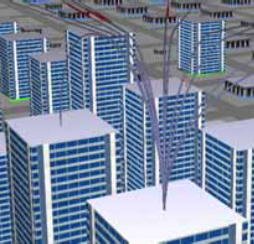
\includegraphics[scale=0.75]{Imagens/evospaces.png}
  	\textsf{\caption[EvoSpaces.]{EvoSpaces \cite{Alam2007}.\label{fig:evospaces}}}
\end{figure}

O EvoSpaces \cite{Alam2007}, mostrado na figura \ref{fig:evospaces}, é uma ferramenta que provê a visualização da arquitetura do software em um ambiente virtual. Aproveita o fato de que os sistemas são, muitas vezes, estruturados hierarquicamente para sugerir o uso de uma metáfora de cidades. As entidades, junto com suas relações, são representadas como glifos residenciais (casa, apartamento, escritório, etc), ao passo que as métricas dessas entidades são exibidas como posições e escalas visuais (tamanho, valor da cor, etc). A ferramenta possui diferentes modos de interação, como \textit{zoom} e capacidades de navegação.

\begin{figure}[htb]
	\centering
  	\frame{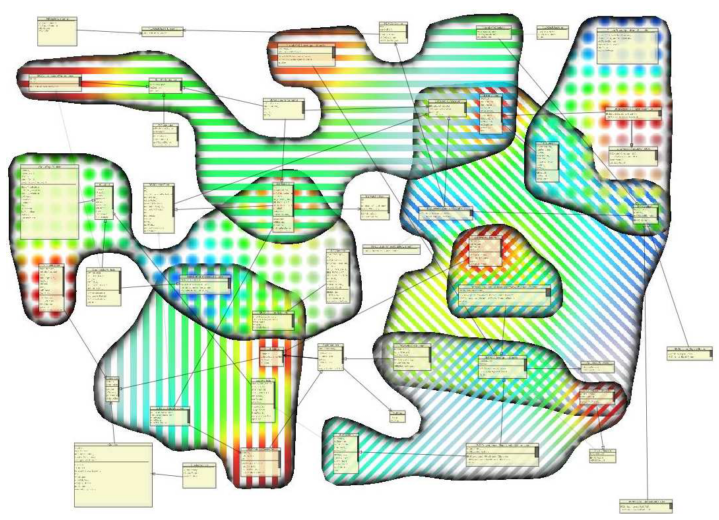
\includegraphics[scale=0.30]{Imagens/areas_of_interest.png}}
  	\textsf{\caption[Areas of Interest.]{Areas of Interest \cite{Byelas2009}.\label{fig:areas-of-interest}}}
\end{figure}

O Areas of Interest \cite{Byelas2009}, mostrado na figura \ref{fig:areas-of-interest}, é uma técnica que consiste em aplicar um algoritmo que agrupa entidades de software com propriedades comuns, as engloba com um contorno e adiciona cores para descrever métricas de software. Para distinguir áreas de sobreposição, cada área tem uma textura diferente, como linhas horizontais, verticais, diagonais e círculos. Além disso, técnicas de sombreamento e transparência são usadas para melhorar a distinção entre várias áreas.

\subsection{Visualização da Evolução da Arquitetura de Software} \label{subsec:visualizacao-evolucao-arquitetura-software}

A evolução de um software tem sido destacada como um dos tópicos mais importantes na engenharia de software \cite{Novais2013}. Trata-se de uma tarefa complexa por gerar grande quantidade de dados e lidar com isso é complicada: estima-se que 60\% do esforço na etapa de manutenção é para entender o software \cite{Corbi1989}. A visualização de software visa ajudar os \textit{stakeholders} a melhorar a compreensão do software, no entanto, elaborar metáforas visuais que representem efetivamente a dimensão tempo com todas as informações relacionadas a evolução do software é uma tarefa difícil \cite{Magnavita2015}.

No contexto da visualização da evolução da arquitetura de um software, um dos grandes desafios, além da quantidade de dados provenientes da evolução, é o crescente tamanho e complexidade do software. Apesar da dificuldade, é importante prover visualizações gerais da arquitetura, dos relacionamentos entre os módulos e das métricas, para cada versão \cite{Khan2012}.

\begin{figure}[htb]
	\centering
  	\frame{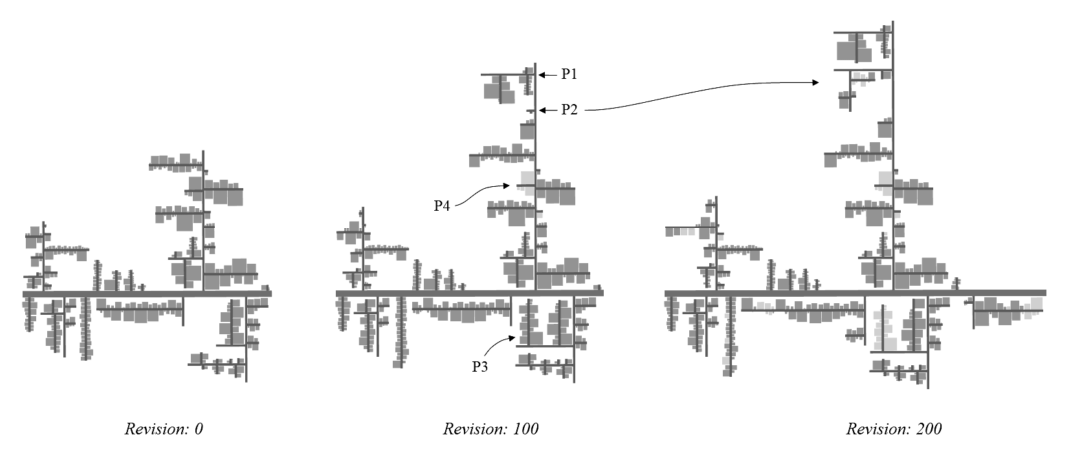
\includegraphics[scale=0.40]{Imagens/crococosmos.png}}
  	\textsf{\caption[CrocoCosmos.]{CrocoCosmos \cite{Steinbruckner2010b}.\label{fig:crococosmos}}}
\end{figure}

O \textit{CrocoCosmos} \cite{Steinbruckner2010b} é um exemplo de ferramenta que utiliza uma metáfora de cidades para representar a evolução estrutural da arquitetura de um software, onde ruas representam pacotes e construções refletem as classes Java. A sequência de representações visuais objetiva destacar as mudanças básicas na estrutura do software, como elementos que foram adicionados, removidos ou movidos dentro da hierarquia. A figura \ref{fig:crococosmos} mostra essa ferramenta. O \textit{Code Flows} \cite{Telea2008} e o \textit{Successive Inheritance Graphs} \cite{Collberg2003} são outros exemplos de visualizações de evolução estrutural de arquitetura de software.

Outra forma de se exibir a evolução de um software é através das suas métricas. Elas encapsulam, sumarizam e provêem informações de qualidade sobre o código-fonte \cite{Langelier2008}. As métricas são essenciais para o entendimento contínuo e para a análise da qualidade do sistema durante todas as fases do seu ciclo de vida \cite{Khan2012}.

O \textit{CodeCity} \cite{Wettel2007} é uma visualização interativa em 3D que avalia a evolução estrutural de sistemas de software e as apresenta utilizando uma metáfora de cidades. As métricas são exibidas através de propriedades visuais dos artefatos da cidade: as propriedades das classes, como o número de métodos e de atributos, são mapeadas como a altura e o tamanho da base das construções, respectivamente; a profundidade dos pacotes é representada através da saturação de cores dos distritos. A figura \ref{fig:codecity} exemplifica essa ferramenta.

\begin{figure}[htb]
	\centering
  	\frame{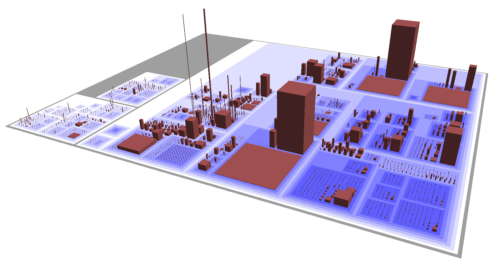
\includegraphics[scale=0.75]{Imagens/codecity.png}}
  	\textsf{\caption[CodeCity.]{Codecity \cite{Wettel2007}.\label{fig:codecity}}}
\end{figure}

Outras soluções que apresentam visualizações da evolução da arquitetura de um software através das métricas são: \textit{The Evolution Matrix} \cite{Lanza2001}, \textit{VERSO} \cite{Langelier2008} e \textit{RelVis} \cite{Pinzger2005}.

\subsection{Estudos Empíricos em Visualização de Software} \label{subsec:estudos-empiricos-visualizacao-software}

As visualizações são importantes para ajudar na compreensão de vários aspectos de um software, além de ajudar a aumentar a produtividade do processo de desenvolvimento, lançando mão de metáforas visuais para representar esses aspectos. Entretanto, não significa que toda visualização de software é útil. Para cada técnica em particular, e para cada intenção de uso, é necessário avaliar a sua utilidade \cite{Diehl2007}. O objetivo principal de uma visualização é transmitir informações de forma compreensível, eficaz e fácil de lembrar. \citeauthor{Diehl2007} agrupa as avaliações das visualizações em dois grupos: quantitativa e qualitativa.

Os métodos quantitativos de avaliação medem propriedades da visualização ou propriedades do usuário interagindo com a visualização. Esse tipo de avaliação requer uma análise estatística dos resultados de um experimento controlado \cite{Diehl2007}.

Já o método qualitativo coleta dados sobre a experiência dos usuários com as visualizações, verbalizados em formato de relatórios. Os métodos qualitativos são de extrema importância quando se trata da percepção humana e da interação com uma visualização \cite{McConathy1993}, incluindo o fato de eles exigirem menos pessoas para o teste e cobrirem mais aspectos da visualização avaliada.

\citeauthor{komlodi2004information}, em sua pesquisa com cerca de 50 estudos de usuários de sistemas de visualização de informação, encontrou quatro áreas de avaliação:
\begin{enumerate}[(i)]
	\item \textit{Experimentos controlados comparando elementos de design}: esses estudos podem comparar elementos específicos;
	\item \textit{Avaliação de usabilidade de uma ferramenta}: esses estudos podem fornecer \textit{feedback} sobre problemas encontrados pelos usuários com uma ferramenta e mostrar como os \textit{designers} podem refinar o \textit{design};
	\item \textit{Experimentos controlados comparando duas ou mais ferramentas}: geralmente tentam comparar novas abordagens com o estado da arte;
	\item \textit{Estudos de caso de ferramentas em contextos realistas}: a vantagem dos estudos de caso é que eles relatam os usuários em seu ambiente natural fazendo tarefas reais, demonstrando viabilidade e utilidade no contexto. A desvantagem é que eles são demorados para conduzir e os resultados podem não ser replicáveis e generalizáveis.
\end{enumerate}

\citeauthor{Seriai2014} realizou um estudo de mapeamento sistemático de métodos de validação em visualização de software. Os autores definiram seis propriedades de classificação desses métodos:
\begin{enumerate}[(i)]
	\item \textit{Tipo de Investigação}: determina qual o tipo de estudo empírico foi usado: experimento, estudo de caso ou questionário;
	\item \textit{Tarefas}: especifica a natureza das tarefas envolvidas na avaliação. Elas são específicas quando o participante tem que resolver um problema específico, ou exploratórias quando o participante não tem uma tarefa específica para executar;
	\item \textit{Fonte de Dados}: caracteriza a fonte dos dados da visualização: industrial, open source e/ou dados domésticos;
	\item \textit{Participantes}: determina o perfil dos participantes usados na avaliação, se houver: estudantes, profissionais ou ambos;
	\item \textit{Medidas}: especifica se a avaliação incluiu medidas objetivas, ou seja, sem ser baseadas no julgamento dos participantes. Caso contrário, as medidas poderiam ser subjetivas ou sem medida
	\item \textit{Referência de Comparação}: define se a ferramenta foi comparada a outras ferramentas.
\end{enumerate}

Como resultados, os autores destacam que 78,16\% dos artigos analisados utilizaram o método de estudo de caso, sendo destes, 65\% puramente análise qualitativa. Além disso, 72,5\% envolviam tarefas específicas na avaliação, 77\% dos artigos usaram ferramentas open source, 70,1\% das avaliações foram realizadas sem participantes. Com relação às medidas, 60,9\% dos trabalhos coletaram medidas objetivas. Por fim, 77\% dos artigos não incluíram nenhuma comparação com outras abordagens. Baseado nesses resultados, os autores concluíram que a análise dos tipos de experimentos feitos mostra uma tendência em relação aos estudos de caso, tarefas específicas, fonte de dados open source, sem participantes, com medidas objetivas e sem referência de comparação \cite{Seriai2014}.

\section{Ferramentas de Análise de Desempenho} \label{sec:ferramentas-analise-desempenho}

O tamanho e a complexidade das aplicações modernas aumentaram a demanda por ferramentas que coletem dados sobre o comportamento dinâmico dos programas, e portanto permitam aos desenvolvedores identificarem gargalos de desempenho nas suas aplicações com um mínimo de esforço. O processo de coleta automática e apresentação dos dados de desempenho de sistemas em execução é chamado de \textit{profiling} \cite{Dmitriev2004}.

Nesse contexto, o \textit{profiling} de \abrv[CPU -- \textit{Central Processing Unit}]{CPU}determina quanto tempo o programa gastou executando várias partes do código. Com isso, se pode calcular o desempenho, em termos de tempo de execução, de determinada funcionalidade ou rotina. Já o \textit{profiling} de memória determina o número, tipos e ciclos de vida dos objetos que o programa aloca \cite{Dmitriev2004}. Existem outras modalidades, no entanto a de CPU e memória são as mais usadas.

Das diferentes técnicas de se realizar o \textit{profiling}, a baseada em instrumentação é a mais comum. Essa técnica trabalha inserindo, ou injetando, trechos especiais de código, chamados de código de instrumentação, na aplicação. A execução desses trechos gera eventos, como entrada/saída de métodos ou alocação de objetos. Esses dados são coletados, processados e, eventualmente, apresentados ao usuário. Com relação ao \textit{profiling} de CPU, essa técnica grava exatamente o número exato de eventos, ao invés de uma aproximação estatística (como acontece com o \textit{profiling} baseado em amostragem) \cite{Dmitriev2004}.

Uma das formas de utilizar o \textit{profiling} baseado em instrumentação é lançando mão do paradigma de programação orientado a aspectos, que permite o aumento da modularidade de um sistema através da separação de interesses. O princípio é que alguma lógica ou funcionalidade possa agir transversalmente entre as diferentes lógicas encapsuladas no sistema usando diferentes tipos de abstrações \cite{Bateman2009}. Para a linguagem de programação Java, o suporte a programação orientada a aspectos é feito usando a biblioteca \textit{AspectJ}.

Existem no mercado várias ferramentas que realizam a medição do atributo de qualidade de desempenho para a linguagem Java. Algumas delas são:
\begin{itemize}
	\item \textit{VisualVM} \cite{Vis}: distribuída gratuitamente com o \textit{Java Development Kit} (JDK), exibe o tempo de execução de cada método em tempo real e o usuário pode, à medida que deseja, tirar fotografias instantâneas da execução do software, os chamados \textit{snapshots};
	\item \textit{JProfiler} \cite{JProfiler}: ferramenta paga, pode exibir o \textit{call graph} de chamadas dos métodos em tempo real, com seus respectivos tempos de execução. Assim como o \textit{VisualVM}, a ferramenta oferece a possibilidade de guardar \textit{snapshots} de determinados momentos da execução;
	\item \textit{YoutKit Java Profiler} \cite{Profiler2016}: ferramenta paga que possui funcionalidades semelhantes às do \textit{JProfiler}.
\end{itemize}

Além das ferramentas de \textit{profiling}, outra maneira de se realizar a análise de desempenho de aplicações é utilizando ferramentas de gerenciamento de desempenho de aplicações, as chamadas APM. Essas ferramentas integram abordagens de mineração de dados de desempenho em ferramentas de monitoramento de desempenho disponíveis no mercado e são frequentemente utilizadas para detectar anomalias no desempenho \cite{Ahmed2016}. Exemplos desse tipo de ferramentas são o \textit{New Relic} \cite{Relic2016}, \textit{AppDynamics} \cite{Appdynamics}, \textit{Dynatrace} \cite{Dynatrace2016} e \textit{Pinpoint} \cite{Pinpoint2016}.

\section{Considerações} \label{sec:consideracoes-cap2}

Os conceitos apresentados neste capítulo são importantes para o entendimento da proposta da seguinte forma. Com relação ao conceito de arquitetura de software, a ferramenta estendida, \textit{PerfMiner}, é focada principalmente na implementação do sistema, e não nos componentes arquiteturais ou relacionamentos entre eles. Além disso, apesar de existirem vários atributos de qualidade, apenas o de desempenho, medido em termos de tempo de execução, é considerado. Com relação aos cenários, é a forma com a qual a avaliação da arquitetura do software é guiada.

A respeito da visualização de software, a extensão proposta utiliza representações visuais para exibir aspectos dinâmicos e de evolução da arquitetura de software. Dessa forma, é exibido o atributo de qualidade de desempenho relacionado a arquitetura do software, além de sua evolução ao longo das versões do sistema. Assim como o \textit{PerfMiner} não trata dos componentes arquiteturais ou dos seus relacionamentos, não são usadas representações visuais para tal fim na extensão.

Foram mencionadas neste capítulo ferramentas de análise de desempenho, como as de \textit{profiling} e APM, pois é possível medir o desempenho de aplicações utilizando-as. Entretanto, há diferenças para a extensão proposta ao \textit{PerfMiner}, principalmente no tocante a identificação da evolução do desempenho. Com relação a técnica de coleta automática de dados, o \textit{PerfMiner} utiliza a instrumentação de código através do \textit{AspectJ}.
	
	% Capitulo 3: Terceiro capítulo (arquivo Includes/Capitulo3.tex)
	% Capíulo 3
\chapter{Estudo sobre a Compatibilidade a Múltiplas Versões da API Android}
\label{ch:estudo}

Este capítulo apresenta o estudo realizado para análise do suporte de aplicações
existentes à múltiplas versões da API da plataforma Android. Foram analisados o
código-fonte de 41 aplicações únicas com o objetivo de identificar e caracterizar
as técnicas de implementação de variabilidades.

O restante do capítulo está organizado da seguinte maneira: 
a seção \ref{sec:objetivos} destaca os objetivos do estudo e as questões de pesquisa.
A seção \ref{sec:aplicacoes-alvo} apresenta os critérios de seleção das aplicações
alvo do estudo, bem como as aplicações selecionadas.
A seção \ref{sec:procedimentos} descreve os procedimentos adotados para responder
cada questão de pesquisa. 
A seção \ref{sec:resultados} apresenta os resultados do estudo, que são discutidos na
seção \ref{sec:discussao}.
Por fim, as ameaças à validade são reportadas na seção \ref{sec:ameacas}.

\section{Objetivos do Estudo e Questões de Pesquisa} \label{sec:objetivos}

Nosso estudo foi realizado com o objetivo de caracterizar, entender e analisar
como as aplicações Android lidam com múltiplas versões da API da plataforma, além
do impacto deste suporte no código-fonte das aplicações. Para atingir este objetivo,
o estudo foi guiado pelas seguintes questões de pesquisa (QPs):

\begin{itemize}
	\item \textbf{QP1}: Quais são as técnicas que aplicações atuais usam para manter
	compatibilidades com as diversas versões da API do Android? O objetivo dessa questão
	é indicar quais as técnicas vem sendo utilizadas e suas características, auxiliando
	desenvolvedores a decidirem o que e quando utilizar em suas aplicações.
		\begin{itemize}
			\item Essa questão foi respondida analisando no código-fonte das aplicações o
			uso de técnicas como: (i) pacotes de compatibilidade, (ii) re-implementação de
			recursos e (iii) acesso explícito às novas API's. Para este último caso,
			aprofundamos a análise para determinar como as aplicações evitam que chamadas
			a novas API's sejam feitas de forma indevida, o que causará uma interrupção na
			execução da aplicação.
		\end{itemize}
	\item \textbf{QP2}: Qual o subconjunto de novas funcionalidades da plataforma que são
	mais utilizadas por aplicações compatíveis com versões antigas da API? Esse levantamento
	auxilia desenvolvedores de aplicações Android a identificar os elementos que eles podem
	utilizar em suas aplicações, permitindo a concentração de esforços nesses elementos.
		\begin{itemize}
			\item Para responder essa questão, contabilizamos os elementos de API's utilizados
			pela aplicação e que são superiores a versão mínima especificado pela mesma. Seja
			através dos pacotes de compatibilidade, da re-implementação de recursos ou do acesso
			explícito às novas API's. Esse elementos foram agrupados pela taxonomia apresentada
			na seção \ref{sec:taxonomia}.
		\end{itemize}
	\item \textbf{QP3}:Qual o esforço necessário para aumentar a compatibilidade com um maior
	número de API's de versões anteriores da plataforma? Estabelecer uma versão elevada de API
	para execução do aplicativo pode significar deixar de atender um grande mercado potencial.
	Assim, a resposta para essa questão dará aos desenvolvedores um indicativo estimado do trabalho
	que terão para aumentar seu mercado potencial.
		\begin{itemize}
			\item Para responder essa questão, modificamos a versão mínima da API e verificamos quais
			novas ocorrências de NewApi são apresentadas pelo Android Lint, de forma a entender o
			esforço em termos de mudanças de código fonte para atender a mesma.
		\end{itemize}
	\item \textbf{QP4}: Qual a incidência de código morto em função da versão da API do Android? 
	A evolução da API mínima exigida pelas aplicações, aqui no sentido de edição da configuração
	no arquivo de manifesto, associada à execução condicional pode resultar em código-morto.
	Analisamos as aplicações para determinar se isso tem ocorrido com frequência e em qual volume.
		\begin{itemize}
			\item Essa questão foi respondida a partir da edição do código-fonte das aplicações.
			Localizamos e removemos todo o código relacionado à qualquer API inferior à mínima
			exigida pela aplicação.
		\end{itemize}
\end{itemize}

\section{Aplicações Alvo de estudo} \label{sec:aplicacoes-alvo}

As aplicações utilizados no estudo são aplicações \textit{open-source} populares,
com um mínimo de 6 mil linhas de código, contabilizados arquivos Java e XML, e de
categorias diversas. Um das aplicações possui 10 mil downloads na Google Play,
outra possui 50 mil \textit{downloads} e as demais mais de 100 mil.

Analisamos um total de 41 aplicações únicas. Não analisamos todas as aplicações em
todas as questões, mas algumas aplicações foram analisadas em mais de uma questão.
Isso ocorreu devido a natureza das nossas questões de pesquisa, que exigiu a análise
de grupos diferentes de aplicações para determinadas questões, com critérios de seleção
adicionais aos citados anteriormente. Assim, definimos 3 grupos de aplicações, apresentados
a seguir.

\subsection{Grupo 1 - Aplicações usando API da plataforma com grande variação de versões}
Aplicações do grupo 1 possuem uma diferença de pelo menos 7 versões entre a API mínima e
a API alvo. A nossa hipótese é que além da aplicação oferecer suporte para versões de API's
antigas também utiliza recursos das versões mais recentes da API quando disponíveis. Tais
aplicações foram utilizadas para responder às questões QP1 e QP2 e são listadas na tabela
\ref{tab:grupo1}. São 25 aplicações nesse grupo.

\begin{table}[!htbp] % TODO posicionar melhor essa tabela
  \centering
  \caption{Aplicações usando API da plataforma com grande variação de versões}
  \begin{tabular}{| l | l | r | r | r | r |}
  	\hline
  	% rótulo das columnas
  	\multicolumn{1}{|c|}{\textbf{Aplicação}} &
  	\multicolumn{1}{c|}{\textbf{Categoria}} &
 	\multicolumn{1}{c|}{\textbf{Downloads}} & 
 	\begin{tabular}[c]{@{}c@{}}
 		\textbf{API}\\ \textbf{Mínima}
 	\end{tabular} &
 	\begin{tabular}[c]{@{}c@{}}\textbf{API}\\ \textbf{Alvo}\end{tabular} &
 	\multicolumn{1}{c|}{\textbf{KLoc}} \\ \hline
 	%dados
 	Wififixer 		& Ferramentas 			& 1.000.000   &  7 & 23 &   9 \\ \hline
 	AnySoftKeyBoard & Ferramentas 			& 1.000.000   &  7 & 23 & 180 \\ \hline
 	Telegram 		& Comunicação 			& 100.000.000 &  9 & 23 & 169 \\ \hline
 	AntennaPod  	& Mídia e Video 		& 100.000 	  & 10 & 23 &  65 \\ \hline
 	Google I/O   	& Livros e Referências 	& 500.000 	  & 14 & 22 &  52 \\ \hline
 	Firefox    		& Comunicação 			& 100.000.000 & 15 & 22 & 233 \\ \hline
 	AnkiDroid     	& Educação 				& 1.000.000   & 10 & 22 &  89 \\ \hline
 	K-9 Mail      	& Comunicação 			& 5.000.000   & 15 & 22 & 117 \\ \hline
 	C:Geo       	& Entretenimento 		& 1.000.000   &  9 & 21 & 123 \\ \hline
 	Zmanim        	& Estilo de Vida 		& 10.000 	  & 10 & 22 &  25  \\ \hline
 	\begin{tabular}[l]{@{}l@{}}
 		Simon Tatham's \\ Puzzles
 	\end{tabular} 	& Quebra-cabeças 		& 100.000 	  &  7 & 23 &   8  \\ \hline
 	Vuze Remote     & Ferramentas			& 100.000	  &  7 & 23 &  20 \\ \hline
 	VLC for Android & 
 	\begin{tabular}[l]{@{}l@{}} Reproduzir e \\
 	 		 editar vídeos \end{tabular}    & 50.000.000  &  8 & 23 &  65 \\ \hline
 	\begin{tabular}[l]{@{}l@{}}
 	 	DuckDuckGo \\ Search \& Stories
 	\end{tabular}   & Livros e referências  & 1.000.000   &  8 & 23 &  23 \\ \hline
 	\begin{tabular}[l]{@{}l@{}}
 		Shattered Pixel \\ Dungeon
 	\end{tabular} 	& RPG 					& 500.000     &  8 & 23 &  58 \\ \hline
 	Persian Calendar& Produtividade			& 100.000 	  &  8 & 23 &  10 \\ \hline
 	Free Mobile Netstat& Ferramentas  		& 100.000 	  &  8 & 23 &   6 \\ \hline
 	MyExpenses    & Finanças 			& 100.000     &  8 & 23 &  80 \\ \hline
    \begin{tabular}[l]{@{}l@{}}
    	Simple Last.fm \\ Scrobbler
    \end{tabular} 	   & Música e áudio     & 500.000     &  7 & 22 &  10 \\ \hline
    Document Viewer	   & Produtividade		& 500.000 	  &  8 & 22 &  77 \\ \hline
	OpenTasks		   & Produtividade      & 100.000     &  8 & 22 &  23 \\ \hline
	\begin{tabular}[l]{@{}l@{}}
		Terminal Emulator \\ for Android
	\end{tabular} 	   & Ferramentas		& 10.000.000  &  4 & 22 &  18 \\ \hline
	ConnectBot		   & Comunicação	    & 1.000.000   &  4 & 22 &  24 \\ \hline
	Quick Dice Roller  & Ferramentas		& 100.000 	  &  4 & 21 &  35 \\ \hline
	\begin{tabular}[l]{@{}l@{}}
		BatteryBot Battery \\ Indicator
	\end{tabular} 	   & Ferramentas		& 5.000.000   &  7 & 22 &  6 \\ \hline
  \end{tabular}
  \label{tab:grupo1}
\end{table}

\subsection{Grupo 2 - Aplicações usando apenas API's mais recentes}
Aplicações do grupo 2 possuem um alto valor de API mínima mas não tem um histórico de suporte
às versões anteriores. Para esse estudo, as versões iguais ou superiores à 16 foram consideradas
como alta. Versões inferiores a esta representam 3.4\% do mercado mundial, conforme pode ser visto
na figura \ref{fig:platform_versions}. E para caracterizar ausência de um histórico de suporte
às versões anteriores,
consideramos aquelas cuja API mínima inicial seja igual ou superior a 11. A nossa hipótese é que
a aplicação foi criada sem a preocupação de oferecer suporte às versões antigas da API o que,
possivelmente, a leva a perder uma fatia do mercado de aplicações. Tais aplicações foram utilizadas
para responder à questão QP3 e estão listadas na tabela \ref{tab:grupo2}. São 10 aplicações nesse grupo.

\begin{table}[!htbp]
  \centering
  \caption{Aplicações usando apenas API's mais recentes}
  \begin{tabular}{| l | l | r | r | r | r |}
  	\hline
  	% rótulo das columnas
  	\multicolumn{1}{|c|}{\textbf{Aplicação}} &
  	\multicolumn{1}{c|}{\textbf{Categoria}} &
 	\multicolumn{1}{c|}{\textbf{Downloads}} & 
 	\begin{tabular}[c]{@{}c@{}}
 		\textbf{API}\\ \textbf{Mínima} \\ \textbf{Inicial}
 	\end{tabular} &
 	\begin{tabular}[c]{@{}c@{}}\textbf{API}\\ \textbf{Mínima}\\ \textbf{Atual}\end{tabular} &
 	\multicolumn{1}{c|}{\textbf{KLoc}} \\ \hline
 	% dados
 	AcDisplay 		& Personalização 		& 1.000.000   & 19 & 16 & 40 \\ \hline
 	Dash Clock		& Personalização		& 1.000.000   & 17 & 17 & 15 \\ \hline
 	Focal (Beta) 	& Fotografia 			& 500.000	  & 16 & 16 &  16 \\ \hline
 	\begin{tabular}[l]{@{}l@{}}
 	 		Hangar - Smart \\ app shortcuts
 	\end{tabular}	& Ferramentas 		& 50.000 	  & 16 & 16 &  12 \\ \hline
 	Indic Keyboard  & Ferramentas 	& 100.000 	  & 14 & 16 &  81 \\ \hline
 	\begin{tabular}[l]{@{}l@{}}
 	 	 	Numix Circle \\ icon pack
 	\end{tabular}   & Personalização    	& 100.000 	  & 11 & 16 &   8 \\ \hline
 	SnoopSnitch     & Ferramentas 			& 100.000     & 14 & 16 &  17 \\ \hline
 	Termux      	& Ferramentas 			& 100.000	  & 21 & 21 &  10 \\ \hline
 	\begin{tabular}[l]{@{}l@{}}
 	 		WiFiAnalyzer \\ (open-source)
 	\end{tabular}   & Ferramentas 			& 100.000     & 22 & 21 &  12 \\ \hline
 	\begin{tabular}[l]{@{}l@{}}
 		Yaac - \\ IRC Client
 	\end{tabular} 	& Ferramentas 			& 50.000 	  & 16 & 16 &  12  \\ \hline
 	\end{tabular}
  \label{tab:grupo2}
\end{table}


\subsection{Grupo 3 - Aplicações usando API's recentes com histórico de uso de API's antigas}
Aplicações do grupo 3 possuem um alto valor de API mínima e também um histórico
de suporte às versões anteriores. Para esse grupo de aplicações, consideramos
aquelas cuja versão da API seja igual ou superior a 15 e a API mínima inicia
menor ou igual a 8. Nossa hipótese é que as aplicações possuem código-morto,
que só seriam executados na presença de API's antigas. Tais aplicações foram
utilizadas para responder à questão QP4 e estão listadas na tabela \ref{tab:grupo3}.
São 7 aplicações nesse grupo.

\begin{table}[!htbp]
  \centering
  \caption{Aplicações usando API's recentes com histórico de uso de API's antigas}
  \begin{tabular}{| l | l | r | r | r | r |}
  	\hline
  	% rótulo das columnas
  	\multicolumn{1}{|c|}{\textbf{Aplicação}} &
  	\multicolumn{1}{c|}{\textbf{Categoria}} &
 	\multicolumn{1}{c|}{\textbf{Downloads}} & 
 	\begin{tabular}[c]{@{}c@{}}
 		\textbf{API}\\ \textbf{Mínima} \\ \textbf{Inicial}
 	\end{tabular} &
 	\begin{tabular}[c]{@{}c@{}}\textbf{API}\\ \textbf{Mínima}\\ \textbf{Atual}\end{tabular} &
 	\multicolumn{1}{c|}{\textbf{KLoc}} \\ \hline
 	% dados
 	AFWall+ 		& Ferramentas	 		& 500.000     & 7  & 15 & 32 \\ \hline
 	aMetro			& 
 	\begin{tabular}[l]{@{}l@{}}
 	 	Mapas e \\ Navegação \end{tabular}	& 100.000	  & 3 & 15 &  10 \\ \hline
 	\begin{tabular}[l]{@{}l@{}}
 	 		Hangar - Smart \\ app shortcuts
 	\end{tabular}	& Ferramentas 		& 50.000 	  & 16 & 16 &   12 \\ \hline
 	K-9 Mail  		& Comunicação 		& 5.000.000	  &  3 & 15 &  117 \\ \hline
 	\begin{tabular}[l]{@{}l@{}}
 	 	 	Orbot Proxy \\ com Tor
 	\end{tabular}   & Comunicação    	& 5.000.000 	  & 4 & 16 & 33 \\ \hline
 	Ringdroid     	&
 	\begin{tabular}[l]{@{}l@{}} Reproduzir e \\
 	 	 	Editar Vídeos \end{tabular}	& 50.000.000	  & 4 & 16 &   6 \\ \hline
 	Transdrone      & Ferramentas 		& 100.000	      & 4 & 15 &  36 \\ \hline
 	\begin{tabular}[l]{@{}l@{}}
 	 		Vanilla Music
 	\end{tabular}   & Música e Áudio 			& 500.000     &  3 & 15 & 25 \\ \hline
 	\end{tabular}
  \label{tab:grupo3}
\end{table}

\section{Procedimentos} \label{sec:procedimentos}

Ter uma visão geral da evolução do atributo de qualidade de desempenho é o objetivo principal desta visualização. Será mostrada a evolução do desempenho entre as versões do sistema, no entanto, destacando também a quantidade total de cenários em cada versão, bem como quantos degradaram e quantos otimizaram o seu desempenho. Serão utilizadas propriedades visuais que simplifiquem a percepção dos desenvolvedores e arquitetos com relação ao desempenho geral do sistema.

Esta visualização ainda está em fase de concepção no momento da escrita desta proposta. Entretanto, sua implementação seguirá a mesma rotina mostrada na figura \ref{fig:funcionamento-geral-visualizacoes}. Planeja-se que esta seja a primeira visualização que o usuário do sistema terá contato, sobretudo por ter granularidade mais alta do que as demais. A partir dela, o usuário poderá navegar entre as outras visualizações descritas neste trabalho.

\section{Resultados do Estudo} \label{sec:resultados}

Através da navegação da visualização de evolução do desempenho, o usuário poderá obter uma sumarização dos cenários de determinada versão do sistema, bem como o desvio de desempenho destes em relação à versão anterior. Nesta visualização, os cenários serão exibidos com propriedades visuais que proporcionem a identificação de quais degradaram e quais otimizaram o desempenho, seus tempos de execução e a porcentagem de desvio.

Esta visualização também está em fase de concepção, assim como a anterior, e sua implementação seguirá igualmente o processo exibido na figura \ref{fig:funcionamento-geral-visualizacoes}. A partir da sumarização, o usuário poderá escolher um dos cenários mostrados e navegar para a visualização do grafo de chamadas.

\section{Discussão} \label{sec:discussao}

Uma das visualizações propostas tem o objetivo de mostrar, para dadas duas versões de um sistema, os métodos que potencialmente causaram o desvio de desempenho para um determinado cenário. Os métodos são exibidos em um grafo direcionado de chamadas com propriedades visuais que destacam quais dos métodos mostrados tiveram desvios de desempenho. É a visualização que possui granularidade mais fina dentre as três propostas como extensão ao \textit{PerfMiner}.

Os grafos podem ser utilizados quando os dados a serem representados são estruturados, ou seja, quando existe uma relação inerente entre os elementos de dados a serem visualizados \cite{Herman2000}. Há uma vasta quantidade de áreas onde os grafos podem ser aplicados, por exemplo: hierarquia de arquivos em formato de árvore, mapas de sites, mapas moleculares e genéticos, diagramas de fluxos de dados, entre outros.

Nesse sentido, em uma chamada de métodos é evidente a relação entre eles, uma vez que os objetos, em um sistema orientado a objetos, trocam mensagens entre si através da invocação dos métodos. O grafo é exibido utilizando o \textit{layout} em árvore, onde os nós filhos estão dispostos abaixo dos nós ancestrais, e a direção dos nós é \textit{bottom-top}. Nesta subseção são apresentadas as propriedades visuais do grafo, o seu funcionamento básico além de um exemplo para exemplificar os grafos.

{\color{red}Adicionar um exemplo da visualização de grafos antes de começar a discorrer sobre as propriedades visuais}

\subsection{Propriedades Visuais} \label{subsec:propriedades-visuais}

{\color{red}Colocar cada elemento visual em subseções}

Juntamente com o grafo de chamadas e seus nós e arestas direcionadas, outras informações foram adicionadas à visualização visando auxiliar os usuários na contextualização do cenário a ser exibido.

\begin{figure}[htb]
   \centering
   \frame{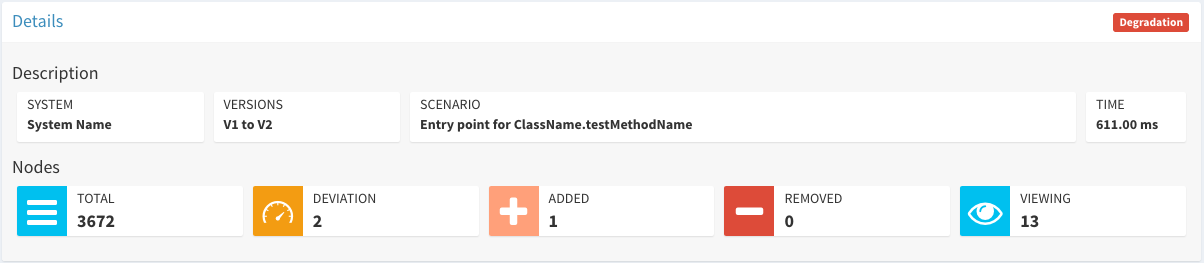
\includegraphics[scale=0.37]{Imagens/detalhes_grafo_chamadas.png}}
   \textsf{\caption[Seção de detalhes do grafo de chamadas.]{Seção de detalhes do grafo de chamadas.\label{fig:detalhes-grafo-chamadas}}}
\end{figure}

Na figura \ref{fig:detalhes-grafo-chamadas}, é mostrada uma visão geral sobre o cenário atual na visualização, contendo informações inerentes ao cenário. Para a seção \textit{Description}, as informações exibidas são:
\begin{itemize}
   \item \textit{System}: nome do sistema analisado;
   \item \textit{Versions}: versões do sistema que foram analisadas. É mostrado no formato \textit{<versionA>} to \textit{<versionB>}. Espera-se que a versão B, neste caso, seja posterior a versão A. No exemplo da figura, a versão V2 (\textit{versionB}) é posterior a versão V1 (\textit{versionA});
   \item \textit{Scenario}: exibe o nome do cenário analisado;
   \item \textit{Time}: mostra o tempo de execução do cenário na versão mais recente. A diferença de tempo entre as duas versões vai guiar o que será exibido na barra de títulos da figura. No exemplo mostrado, o tempo na última versão degradou com relação ao tempo na versão anterior, sendo exibido, no canto superior direito, um rótulo em vermelho marcando o cenário como degradado (\textit{degradation}). Caso o tempo do cenário seja otimizado, é exibido um rótulo verde marcando-o como otimizado (\textit{optimization}).
\end{itemize}

Para a seção \textit{Nodes}, as informações são as seguintes:
\begin{itemize}
   \item \textit{Total}: mostra o número total de nós do cenário. Vale salientar que cada nó representa um método executado durante a hierarquia de chamadas do cenário. Pode acontecer de nós diferentes representarem o mesmo método. Isso pode acontecer porque o mesmo método pode ser chamado hierarquias de chamadas diferentes;
   \item \textit{Deviation}: exibe o número de nós que tiveram algum desvio de desempenho. Para que um determinado nó seja considerado com desvio de desempenho, ele (i) tem que estar presente nas duas versões analisadas e (ii) tenha ocorrido diferenças, para mais ou para menos, no seu desempenho durante a execução do cenário nas versões analisadas;
   \item \textit{Added}: apresenta o número de nós que foram adicionados da versão anterior para a posterior. Ou seja, são os nós que não existiam na execução do cenário para a versão anterior e passaram a existir na execução da versão posterior;
   \item \textit{Removed}: o contrário do conceito anterior. São apresentados os nós que foram removidos da versão anterior para a posterior. Os nós removidos não são exibidos na visualização do grafo de chamadas;
   \item Viewing: apresenta a quantidade de nós que estão sendo mostrados no grafo de chamadas.
\end{itemize}

A segunda parte da visualização é o grafo de chamadas propriamente dito. Esse grafo, como mencionado, é composto de nós e arestas direcionadas que expõem os caminhos das chamadas dos métodos para o cenário analisado. Os nós, representados por caixas, possuem algumas características visuais, apresentadas adiante.

\begin{figure}[htb]
   \centering
   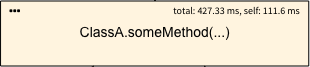
\includegraphics[scale=0.70]{Imagens/no_sem_desvio.png}
   \textsf{\caption[Nó que representa um método sem desvio de desempenho.]{Nó que representa um método sem desvio de desempenho.\label{fig:no-sem-desvio}}}
\end{figure}

O primeiro e mais básico tipo de nó é o que representa um método que não teve desvios de desempenho para o cenário e versões analisadas, apresentado na figura \ref{fig:no-sem-desvio}. As características desse nó são:\tabularnewline
\begin{itemize}
   \item \textit{Cor}: esta é a principal característica que diferencia os nós uns dos outros. No caso deste nó, a cor é marrom claro;
   \item \textit{Nome do nó}: posicionado ao centro, são mostrados o nome da classe e o nome do método executado, no formato \textit{ClassName.methodName()}. Para otimizar e evitar a exibição de grande quantidade de texto, o nome do pacote e os parâmetros do método foram ocultados, sendo estes representados por três pontos (...). Essa definição serve para todos os tipos de nós dessa visualização;
   \item \textit{Tempos de execução}: localizados no canto superior direito do nó, são apresentados dois tempos de execução: à esquerda, o tempo total do nó, que representa a soma dos tempos de execução dos nós filhos com o tempo do próprio nó. No exemplo da figura, o tempo total foi de 427,33 milissegundos; e à direita, o tempo do próprio nó, desconsiderando o tempo dos nós filhos. Na figura, o tempo foi de 111,6 milissegundos;
   \item \textit{Detalhes}: no canto superior esquerdo é exibido um ícone onde, ao passar o cursor do mouse, o usuário pode obter mais informações sobre o nó. No caso de um nó sem desvio de desempenho, as informações exibidas nesta seção são o nome do pacote e os parâmetros do método, se houver. A figura \ref{fig:detalhes-no-sem-desvio} a seguir mostra essa seção.
\end{itemize}

\begin{figure}[htb]
   \centering
   \frame{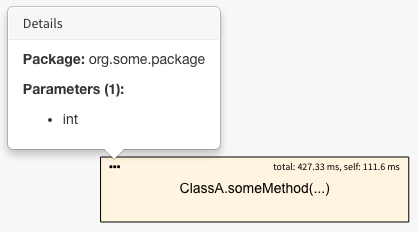
\includegraphics[scale=0.65]{Imagens/detalhes_no_sem_desvio.png}}
   \textsf{\caption[Seção de detalhes do nó sem desvio de desempenho.]{Seção de detalhes do nó sem desvio de desempenho.\label{fig:detalhes-no-sem-desvio}}}
\end{figure}

Quando um cenário possui nós que otimizaram o seu desempenho em relação à execução para a versão anterior, outros elementos visuais são acrescidos à visualização. A figura \ref{fig:no-otimizado} a seguir apresenta um nó otimizado:

\begin{figure}[htb]
   \centering
   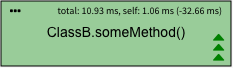
\includegraphics[scale=0.70]{Imagens/no_otimizado.png}
   \textsf{\caption[Nó que representa um método com otimização de desempenho.]{Nó que representa um método com otimização de desempenho.\label{fig:no-otimizado}}}
\end{figure}

As características visuais deste nó, além das comentadas anteriormente, são:
\begin{itemize}
   \item \textit{Cor}: os nós que otimizaram o atributo de qualidade desempenho são mostrados em um tom de verde;
   \item \textit{Tempos de execução}: além dos tempos total e do próprio nó, um nó com desvio de desempenho, seja otimização ou degradação, apresenta a diferença entre os tempos de execução da versão anterior para a posterior entre parênteses, no canto superior direito. No exemplo da figura, o nó melhorou o seu tempo em 32,66 milissegundos;
   \item \textit{Setas}: no canto inferior direito são mostradas setas indicativas de quão forte ou fraca foi a variação de desempenho. No caso de nós com otimização, são exibidas setas verdes apontadas para cima, onde cada uma delas representa 25\% de desvio do tempo com relação à versão anterior. Sendo assim, uma única seta representa um desvio de 0 a 25\%, duas setas de 25\% a 50\%, três setas de 50\% a 75\% e quatro setas de 75\% ou superior. No exemplo apresentado na figura \ref{fig:no-otimizado}, a otimização se deu entre 50\% e 75\% do desempenho anterior;
   \item \textit{Detalhes}: esta seção para os nós com otimização de desempenho possui informações diferentes das relatadas anteriormente, como podem ser vistas na figura \ref{fig:detalhes-no-otimizado}. Além das informações sobre o pacote e os parâmetros, também são apresentadas sobre os tempos de execução da versão anterior e posterior, além da variação de tempo.
\end{itemize}

\begin{figure}[htb]
   \centering
   \frame{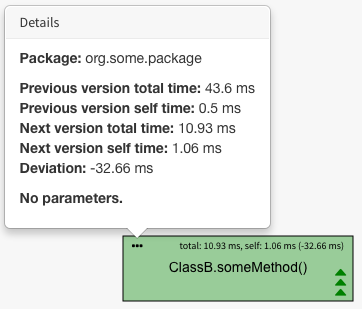
\includegraphics[scale=0.65]{Imagens/detalhes_no_otimizado.png}}
   \textsf{\caption[Seção de detalhes do nó com otimização de desempenho.]{Seção de detalhes do nó com otimização de desempenho.\label{fig:detalhes-no-otimizado}}}
\end{figure}

 A visualização também é capaz de apontar se determinado nó teve o seu desempenho degradado com relação à versão anterior. A figura \ref{fig:no-degradado} apresenta um nó degradado:

\begin{figure}[htb]
   \centering
   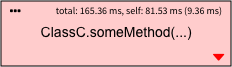
\includegraphics[scale=0.70]{Imagens/no_degradado.png}
   \textsf{\caption[Nó que representa um método com degradação de desempenho.]{Nó que representa um método com degradação de desempenho.\label{fig:no-degradado}}}
\end{figure}

As características visuais deste nó são bem semelhantes às apresentadas para os nós otimizados:
\begin{itemize}
   \item \textit{Cor}: os nós que degradaram o desempenho são mostrados em vermelho claro;
   \item \textit{Tempos de execução}: também são exibidos os tempos de execução total, do próprio nó e o desvio de desempenho. No exemplo, o nó degradou o tempo em 9,36 milissegundos;
   \item \textit: as setas indicativas de variação de desempenho para nós de degradação são apontadas para baixo, de cor vermelha. No exemplo, a degradação se deu entre 0 e 25\% do desempenho anterior;
   \item \textit{Detalhes}: esta seção possui as mesmas informações dos nós relatados até aqui, como podem ser vistas na figura \ref{fig:detalhes-no-degradado} a seguir.
\end{itemize}

\begin{figure}[htb]
   \centering
   \frame{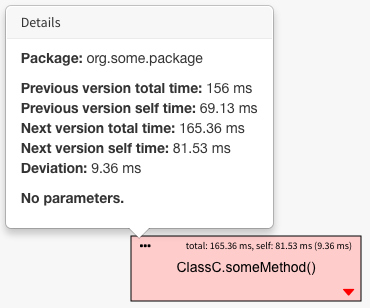
\includegraphics[scale=0.65]{Imagens/detalhes_no_degradado.png}}
   \textsf{\caption[Seção de detalhes do nó com degradação de desempenho.]{Seção de detalhes do nó com degradação de desempenho.\label{fig:detalhes-no-degradado}}}
\end{figure}

Um cenário pode apresentar, para diferentes versões, nós de chamadas de métodos que estão presentes na versão posterior, mas que não existiam na versão anterior. A visualização representa esses nós como mostra a figura \ref{fig:no-adicionado}. A descrição dos atributos visuais é a que segue:

\begin{figure}[htb]
   \centering
   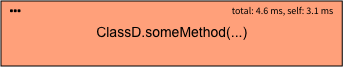
\includegraphics[scale=0.70]{Imagens/no_adicionado.png}
   \textsf{\caption[Nó que representa um método adicionado.]{Nó que representa um método adicionado.\label{fig:no-adicionado}}}
\end{figure}

\begin{itemize}
   \item \textit{Cor}: os nós que degradaram o desempenho são mostrados na cor salmão claro;
   \item \textit{Tempos de execução}: os tempos de execução total e do próprio nó são exibidos. No exemplo, o nó tem tempo total de em 4,6 milissegundos e o seu tempo é de 3,1 milissegundos.
   \item \textit{Detalhes}: nos nós adicionados, os detalhes possuem as mesmas informações exibidas para os nós de degradação ou de otimização. No entanto, uma mensagem é exibida em vermelho indicando que o nó adicionado é um potencial causador da degradação de desempenho do cenário. A figura \ref{fig:detalhes-no-adicionado} adiante apresenta esta seção.
\end{itemize}

\begin{figure}[htb]
   \centering
   \frame{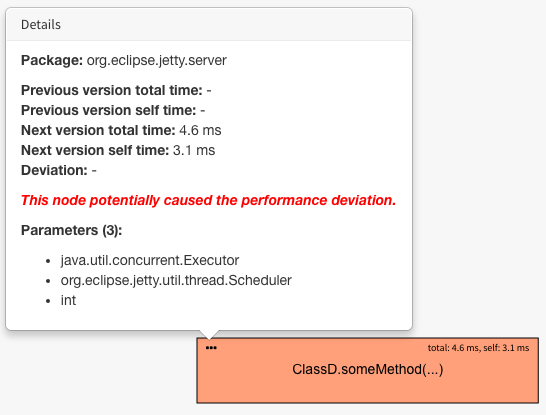
\includegraphics[scale=0.65]{Imagens/detalhes_no_adicionado.png}}
   \textsf{\caption[Seção de detalhes do nó adicionado.]{Seção de detalhes do nó adicionado.\label{fig:detalhes-no-adicionado}}}
\end{figure}

Além dos que representam métodos com ou sem desvio de desempenho, e métodos adicionados, há um tipo de nó que representa um agrupamento de vários outros: o agrupado. Assim, os que não estão diretamente relacionados com nós de desvio ou adicionados, são omitidos e representados por um único nó agrupado. A figura \ref{fig:no-agrupamento} a seguir ilustra esse tipo de nó, seguido da descrição dos seus atributos visuais.

\begin{figure}[htb]
   \centering
   \frame{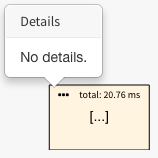
\includegraphics[scale=0.70]{Imagens/no_agrupamento.png}}
   \textsf{\caption[Nó que representa um agrupamento de outros nós.]{Nó que representa um agrupamento de outros nós.\label{fig:no-agrupamento}}}
\end{figure}

\begin{itemize}
   \item \textit{Cor}: os nós de agrupamento são mostrados na cor marrom claro;
   \item \textit{Nome do nó}: posicionado ao centro, é exibido o texto \textit{[...]};
   \item \textit{Tempos de execução}: é exibido o tempo de execução total que representa a soma de todos os tempos de execução dos nós contidos no agrupamento. No exemplo, o tempo total é de 20,76 milissegundos;
   \item \textit{Detalhes}: como pode ser percebido na imagem, este tipo de nó não possui detalhes a serem apresentados.
\end{itemize}

As propriedades visuais apresentadas para a visualização do grafo de chamadas incluem, em suma, duas partes: (i) seção de detalhes, contendo informações gerais sobre o cenário; e (ii) seção do grafo de chamadas, onde a execução dos métodos é representada através de nós e arestas. Esta seção é a mais importante desta visualização, contendo características visuais que diferem os nós de acordo com sua classificação. Um resumo dessas características é apresentado na tabela \ref{tab:resumo-caracteristicas-nos} a seguir.

\begin{table}[!htb]
   \textsf{\caption{Resumo das características visuais dos nós.\label{tab:resumo-caracteristicas-nos}}}
   \centering
   \medskip
   \begin{tabular}{c|c|c|c|c}
   \textbf{Tipo} & \textbf{Cor}   & \textbf{\begin{tabular}[c]{@{}c@{}}Tempos de\\ Execução\end{tabular}} & \textbf{Setas}                                                  & \textbf{Detalhes}                                                                     \\ \hline
   Sem desvio    & Marrom claro   & Total e próprio                                                       & Sem setas                                                       & \begin{tabular}[c]{@{}c@{}}Pacotes e \\ parâmetros\end{tabular}                       \\ \hline
   Degradado     & Vermelho claro & \begin{tabular}[c]{@{}c@{}}Total, próprio\\ e desvio\end{tabular}     & \begin{tabular}[c]{@{}c@{}}Vermelhas,\\ para baixo\end{tabular} & \begin{tabular}[c]{@{}c@{}}Pacotes, tempos\\ de execução e \\ parâmetros\end{tabular} \\ \hline
   Otimizado     & Verde claro    & \begin{tabular}[c]{@{}c@{}}Total, próprio\\ e desvio\end{tabular}     & \begin{tabular}[c]{@{}c@{}}Verdes,\\ para cima\end{tabular}     & \begin{tabular}[c]{@{}c@{}}Pacotes, tempos\\ de execução e \\ parâmetros\end{tabular} \\ \hline
   Adicionado    & Salmão claro   & Total e próprio                                                       & Sem setas                                                       & \begin{tabular}[c]{@{}c@{}}Pacotes, tempos\\ de execução e \\ parâmetros\end{tabular} \\ \hline
   Agrupado      & Marrom claro   & Total                                                                 & Sem setas                                                       & Sem detalhes
   \end{tabular}
\end{table}

\subsubsection{Interação} \label{subsec:interacao}

Esta visualização exibe um conjunto de informações que a torna capaz de indicar os métodos que potencialmente foram responsáveis por desvios de desempenho de um determinado cenário. Contudo, o usuário pode interagir com o grafo: (i) obtendo mais informações sobre um nó, passando o cursor do \textit{mouse} por cima do ícone de detalhes, como mostrado anteriormente; e (ii) executando o efeito de \textit{zoom} sobre o grafo para afastar ou aproximar a visualização. Esse efeito pode fazer com que o grafo seja comportado novamente na área de desenho.

\subsection{Funcionamento} \label{subsec:funcionamento-visualizacao-3}

A visualização utiliza os artefatos de saída gerados após a execução completa do \textit{PerfMiner}, de modo que se configura como mais uma etapa da ferramenta. A figura \ref{fig:perfminer-fase4} ilustra essa etapa. A extensão foi implementada em uma aplicação web, conforme explanado anteriormente e ilustrado na figura \ref{fig:funcionamento-geral-visualizacoes}. Embora o funcionamento mostrado nessa figura seja geral, são necessários processamentos específicos para esta visualização, a fim de tratar os dados para serem exibidos para o usuário.

Para esta visualização, seguindo o funcionamento mostrado na figura \ref{fig:funcionamento-geral-visualizacoes}, o usuário realiza a requisição para esta visualização, passando como parâmetros o nome do sistema e as duas versões (passo 1). Os passos 2 e 3, em detalhes, é exibido na figura \ref{fig:passos-2-3-grafo-chamadas}.

\begin{figure}[!htb]
   \centering
   \frame{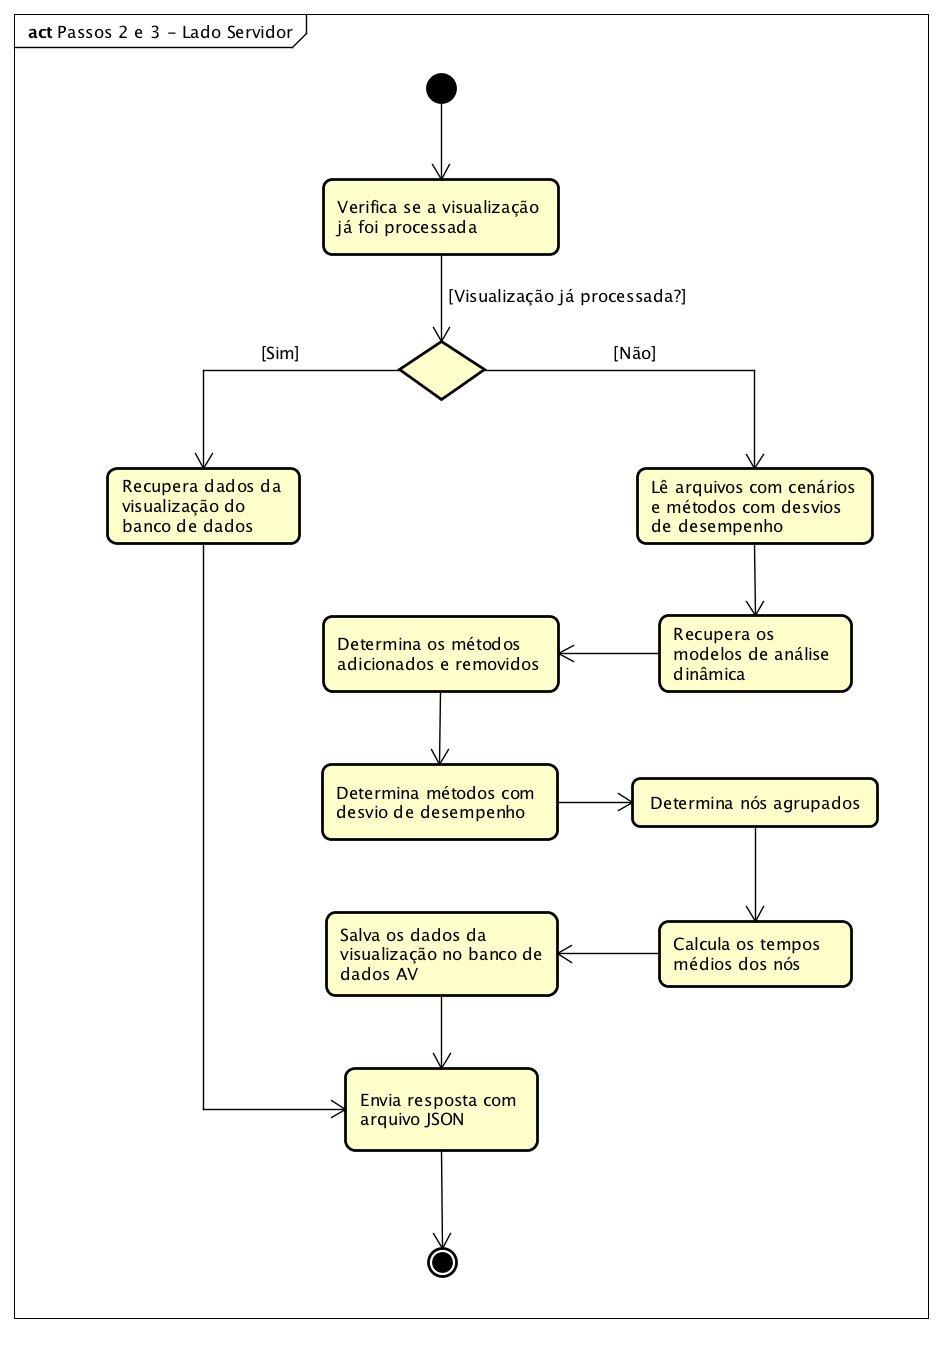
\includegraphics[scale=0.45]{Imagens/visualizacao_3_fase_2_e_3.png}}
   \textsf{\caption[Passos 2 e 3 da visualização grafo de chamadas.]{Passos 2 e 3 da visualização grafo de chamadas.\label{fig:passos-2-3-grafo-chamadas}}}
\end{figure}

O processo se inicia quando o servidor recebe a requisição do usuário, solicitando a visualização do grafo de chamadas para determinadas versões de um sistema. Ao receber, a aplicação verifica se a visualização requerida já foi processada anteriormente, consultando-a no banco de dados QAV. Em caso positivo, os dados são recuperados, o arquivo JSON é montado e enviado na resposta do servidor, e o processo acaba.

Caso a visualização ainda não tenha sido processada, os arquivos de saída do \textit{PerfMiner} contendo informações sobre os cenários e métodos com desvio de desempenho são lidos e os modelos de análise dinâmica de ambas as versões são recuperados do banco de dados DAM. Esse modelo é formado por um grafo com todos os nós de chamadas dinâmico que representa cada execução do cenário.

De posse dos nós recuperados, são determinados os métodos que foram adicionados ou removidos comparando os nós da versão atual com os da anterior. Depois disso, a partir dos métodos indicados pelos arquivos de saída do \textit{PerfMiner}, são determinados os nós com desvios de desempenho, seja degradação ou otimização.

Na extensão, os nós identificados como adicionados e com desvio são candidatos a serem exibidos. Optou-se por apresentar apenas os nós com desvio, nós adicionados e alguns nós sem desvio de desempenho, mas que garantem o entendimento do grafo, de modo que poucos nós são renderizados no navegador do usuário. Essa decisão levou em consideração a quantidade de nós de um cenário, que facilmente pode passar dos milhares, o desempenho da própria aplicação web e a eficácia no entendimento da visualização por parte do usuário. Espera-se que, com menos nós exibidos, os usuários consigam entender e acompanhar mais claramente a evolução do atributo de qualidade de desempenho.

Após determinar os nós com desvios de desempenho, são criados nós de agrupamento para representar os nós que não serão exibidos na visualização. Depois disso, os tempos médios dos nós a serem exibidos são calculados, levando em consideração todas as ocorrências do método no cenário. Após, os dados do processamento são salvos no banco de dados QAV e, por fim, o arquivo JSON que dá suporte à visualização é montado e enviado como resposta do servidor, e o processo acaba.

Quando o usuário recebe a resposta, há um procedimento executado no seu navegador, que recebe e processa o arquivo JSON e, ao final, renderiza o grafo de chamadas. Esse processo representa o passo 5 da figura \ref{fig:funcionamento-geral-visualizacoes} está exposto em detalhes na figura \ref{fig:passo-5-grafo-chamadas} adiante. O início ocorre ao receber o arquivo do servidor e a primeira atividade é criar a área de desenho que abrigará o grafo. Nessa atividade são considerados a altura e largura do monitor do usuário, de modo que a área útil de apresentação seja compatível com a área do monitor.

\begin{figure}[!htb]
   \centering
   \frame{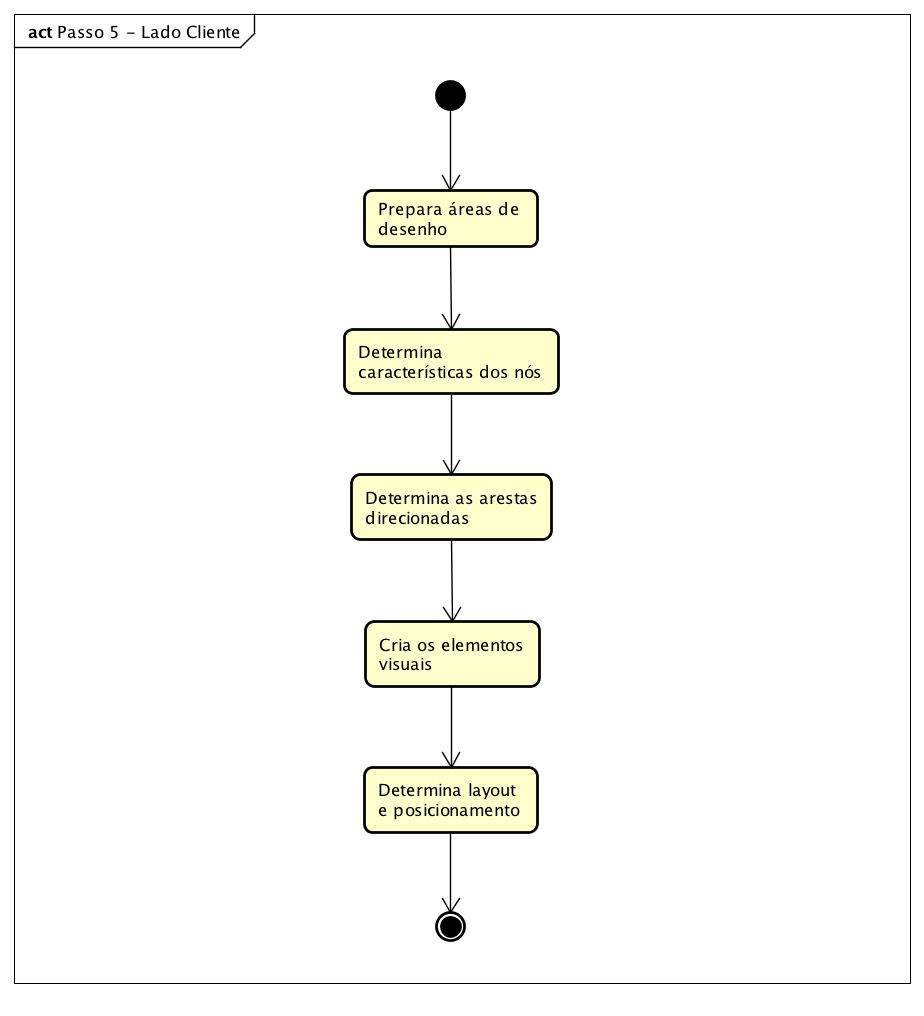
\includegraphics[scale=0.50]{Imagens/visualizacao_3_fase_5.png}}
   \textsf{\caption[Passos 5 da visualização grafo de chamadas.]{Passos 5 da visualização grafo de chamadas.\label{fig:passo-5-grafo-chamadas}}}
\end{figure}

Após isso, as características dos nós contidos no arquivo JSON são determinadas. Para cada um deles, são determinados: (i) a altura e largura da sua caixa, que é diretamente proporcional ao tamanho do nome a ser exibido. Vale salientar que o pacote da classe é omitido para a exibição do nome; (ii) a cor, que depende do seu tipo; (iii) os tempos de execução total e, caso pertinente, o do próprio nó e o de desvio; (iv) as setas, que dependem do seu tipo e da porcentagem de desvio do tempo de execução ocorrida de uma versão para outra; e (v) os detalhes, que dependem do tipo do nó.

Depois, as arestas são determinadas de acordo com a relação de nós pais e filhos contidos no arquivo. Elas são direcionadas do nó pai para os filhos, indicando a hierarquia de chamadas.

Com a definição dos nós e suas características, e das arestas, a próxima atividade do processo é criar os elementos visuais na área de desenho, para, posteriormente, determinar o \textit{layout} (conforme citado anteriormente, o \textit{layout} utilizado é em árvore) e posicionamento dos nós. Por fim, o grafo de chamadas é renderizado para o usuário.

\subsection{Exemplo de Uso da Ferramenta: Jetty} \label{subsec:exemplo-uso-jetty}

Foi realizado um estudo de caso para exemplificar o uso das visualizações. Para tanto, foi utilizado duas versões da aplicação Jetty \cite{Jetty2016}: 9.2.6 e 9.3.0.M1. Esse sistema faz parte do Projeto Eclipse e é um \textit{framework open-source} que provê um servidor web além de um servlet container Java. Essa aplicação foi escolhida para o estudo de caso pois todos os tipos de nós foram capazes de ser exemplificados.

Para a primeira fase do \textit{PerfMiner}, a análise dinâmica, todos os testes automatizados foram considerados cenários. Como os testes são implementados em JUnit 4, o aspecto interceptou todos os métodos marcados com a anotação \texttt{@Test} como métodos de entrada de um cenário. A análise dinâmica, como mencionado anteriormente, foi executada no mesmo computador para ambas as versões, nas mesmas condições e com todos os serviços não essenciais desabilitados. A suíte de testes do Jetty foi executada 30 vezes para que as medições de desempenho fossem mais precisas em termos de tempo de execução \cite{Pinto2015}.

A resultado da análise foi um total de 11 cenários, sendo 7 com degradação do desempenho e 4 com otimização. No grafo gerado, é possível que dois nós representem o mesmo método, indicando duas execuções, e as arestas direcionadas representam invocações entre os métodos. A figura \ref{fig:exemplo-degradacao} exemplifica o grafo de um cenário com degradação.

\begin{figure}[!htb]
   \centering
   \frame{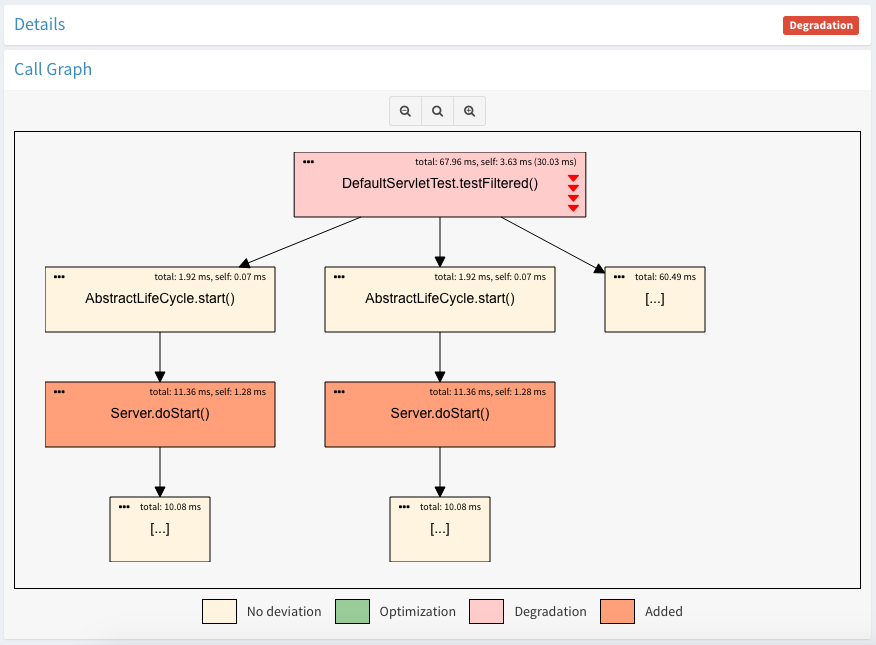
\includegraphics[scale=0.52]{Imagens/exemplo_degradacao.png}}
   \textsf{\caption[Grafo de chamadas de um cenário com degradação de desempenho.]{Grafo de chamadas de um cenário com degradação de desempenho.\label{fig:exemplo-degradacao}}}
\end{figure}

O grafo exibido destaca que o nó raiz, \texttt{DefaultServletTest.testFiltered()}, teve uma degradação de desempenho de mais de 75\%, indicado pela cor do nó, vermelho claro, e pelas quatro setas vermelhas para baixo. É possível notar também que dois nós que representam o método \texttt{Server.doStart()} foram adicionados. Isso significa que durante a execução do cenário \texttt{Entry point for DefaultServletTest.testFiltered} duas chamadas a esse método foram efetuadas na versão 9.3.0.M1, e elas não existiam na versão 9.3.6. Os nós adicionados são indicados como potenciais causadores de degradação de desempenho, de modo que, possivelmente, esses nós influenciaram na degradação do raiz. Na visualização há nós que não têm relação com os desvios, representados como agrupados, e nós sem desvio, representados na cor marrom claro.

Na mesma figura, além do próprio grafo, na parte superior da seção \textit{Call Graph} é encontrada uma barra de ferramentas com botões de \textit{Zoom Out}, \textit{Zoom to Fit} e \textit{Zoom In}; e na parte inferior é exibida uma legenda ajudando os usuários a identificarem os nós do grafo. Os botões de \textit{zoom} e a legenda são exibidos para todos os grafos, independente da quantidade de nós ou do tipo de desvio ocorrido.

Na figura \ref{fig:exemplo-detalhes-degradacao} adiante, a seção \textit{Details} desse cenário é exibida expandida, indicando, no rótulo, que o cenário teve o seu desempenho degradado entre as versões, e que o total de nós para esse cenário foi de 1695.

\begin{figure}[!htb]
   \centering
   \frame{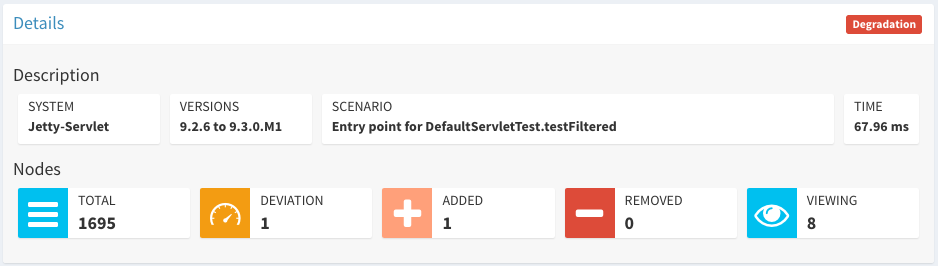
\includegraphics[scale=0.48]{Imagens/exemplo_detalhes_degradacao.png}}
   \textsf{\caption[Detalhes de um cenário com degradação de desempenho.]{Detalhes de um cenário com degradação de desempenho.\label{fig:exemplo-detalhes-degradacao}}}
\end{figure}

A figura \ref{fig:exemplo-otimizacao} a seguir apresenta o cenário \texttt{Entry point for ServletContextHandler\\Test.testFallThrough} com otimização de desempenho. Dois nós contribuíram para esse desvio, identificados pela cor verde claro: \texttt{Server.doStart()} e \texttt{ServletContextHandler.\\relinkHandlers()}. No primeiro, a variação foi entre 50\% e 75\%, ao passo que no segundo foi de mais de 75\%. Há ainda a representação de nós agrupados e sem desvio.

\begin{figure}[!htb]
   \centering
   \frame{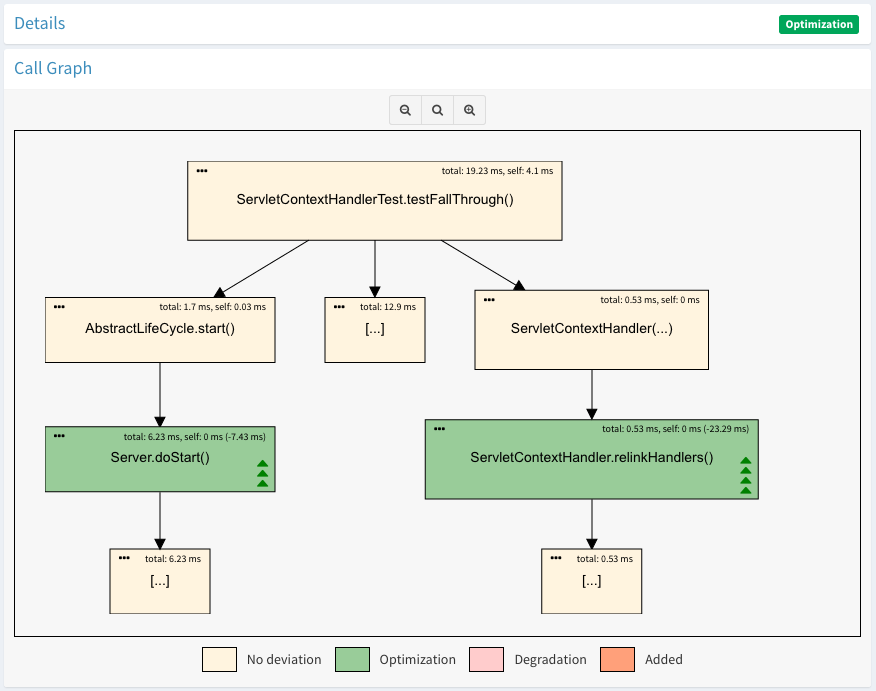
\includegraphics[scale=0.52]{Imagens/exemplo_otimizacao.png}}
   \textsf{\caption[Grafo de chamadas de um cenário com otimização de desempenho.]{Grafo de chamadas de um cenário com otimização de desempenho.\label{fig:exemplo-otimizacao}}}
\end{figure}

\begin{figure}[!htb]
   \centering
   \frame{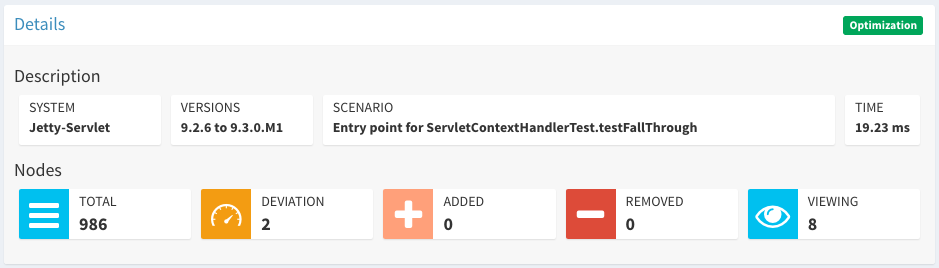
\includegraphics[scale=0.48]{Imagens/exemplo_detalhes_otimizacao.png}}
   \textsf{\caption[Detalhes de um cenário com otimização de desempenho.]{Detalhes de um cenário com otimização de desempenho.\label{fig:exemplo-detalhes-otimizacao}}}
\end{figure}

A seção \textit{Details} expandida pode ser vista na figura \ref{fig:exemplo-detalhes-otimizacao}. O rótulo de otimização é exibido no canto superior esquerdo indicando o tipo de desvio ocorrido no cenário. A figura indica um total de 986 nós para esse cenário.

A tabela \ref{tab:jetty-v9.2.6-v9.3.0.M1} a seguir mostra uma lista com todos os cenários para o sistema Jetty, versões 9.2.6 para 9.3.0.M1. Nela, são exibidas as porcentagens de desvio de degradação ou otimização para os cenários.

\begin{sidewaystable}[!htb]
   \textsf{\caption{Cenários para o Jetty, versões 9.2.6 para 9.3.0.M1.\label{tab:jetty-v9.2.6-v9.3.0.M1}}}
   \centering
   \medskip
   \begin{tabular}{l|c|c|c|c}
   \multicolumn{1}{c|}{\textbf{Nome}}                                                                                                       & \textbf{\begin{tabular}[c]{@{}c@{}}Tempo \\ v9.2.6 (ms)\end{tabular}} & \textbf{\begin{tabular}[c]{@{}c@{}}Tempo \\ v9.3.0.M1 (ms)\end{tabular}} & \textbf{\begin{tabular}[c]{@{}c@{}}Variação \\ (\%)\end{tabular}} & \textbf{\begin{tabular}[c]{@{}c@{}}Tipo de \\ Desvio\end{tabular}} \\ \hline
   \begin{tabular}[c]{@{}l@{}}Entry point for \\ DispatcherForwardTest.testQueryRetainedByForward\\ WithoutQuery\end{tabular}              & 569,26                                                                & 597,33                                                                   & 4,93                                                              & Degradação                                                         \\ \hline
   \begin{tabular}[c]{@{}l@{}}Entry point for \\ SSLAsyncIOServletTest.testAsyncIOWritesWith\\ Aggregation\end{tabular}                    & 549,21                                                                & 587,55                                                                   & 6,98                                                              & Degradação                                                         \\ \hline
   \begin{tabular}[c]{@{}l@{}}Entry point for \\ AsyncServletLongPollTest.testSuspendedRequest\\ CompletedByAnotherRequest\end{tabular}    & 620,36                                                                & 634,60                                                                   & 2,29                                                              & Degradação                                                         \\ \hline
   Entry point for DefaultServletTest.testFiltered                                                                                         & 37,93                                                                 & 67,96                                                                    & 79,17                                                             & Degradação                                                         \\ \hline
   \begin{tabular}[c]{@{}l@{}}Entry point for \\ ServletContextHandlerTest.testReplaceServlet\\ HandlerWithoutServlet\end{tabular}         & 429,60                                                                & 453,96                                                                   & 5,67                                                              & Degradação                                                         \\ \hline
   \begin{tabular}[c]{@{}l@{}}Entry point for \\ AsyncContextListenersTest.testAsyncDispatch\\ AsyncCompletePreservesListener\end{tabular} & 601,83                                                                & 622,96                                                                   & 3,51                                                              & Degradação                                                         \\ \hline
   \begin{tabular}[c]{@{}l@{}}Entry point for \\ AsyncIOServletTest.testAsyncWriteThrowsError\end{tabular}                                 & 599,10                                                                & 611,00                                                                   & 1,98                                                              & Degradação                                                         \\ \hline
   \begin{tabular}[c]{@{}l@{}}Entry point for \\ DispatcherForwardTest.testQueryAggregatesWith\\ FormByForwardWithoutQuery\end{tabular}    & 26,46                                                                 & 20,76                                                                    & 21,54                                                             & Otimização                                                         \\ \hline
   \begin{tabular}[c]{@{}l@{}}Entry point for \\ ServletContextHandlerTest.testFallThrough\end{tabular}                                    & 52,00                                                                 & 19,23                                                                    & 63,01                                                             & Otimização                                                         \\ \hline
   \begin{tabular}[c]{@{}l@{}}Entry point for \\ AsyncContextListenersTest.testListenerCleared\\ OnSecondRequest\end{tabular}              & 23,90                                                                 & 17,16                                                                    & 28,20                                                             & Otimização                                                         \\ \hline
   \begin{tabular}[c]{@{}l@{}}Entry point for \\ ServletContextHandlerTest.testAddServletAfterStart\end{tabular}                           & 55,56                                                                 & 20,40                                                                    & 63,28                                                             & Otimização                                                     
   \end{tabular}
\end{sidewaystable}

A maior variação absoluta foi para o cenário \texttt{Entry point for DefaultServletTest\\.testFiltered}, uma degradação de 79,17\%. Como destacado na figura \ref{fig:exemplo-degradacao}, dois nós com tempos significantes com relação ao cenário foram adicionados, provavelmente, causando a degradação. O gráfico \ref{fig:grafico-jetty-v9.2.6-v9.3.0.M1} adiante exibe a porcentagem de variação de desempenho.

\begin{sidewaysfigure}[!htb]
   \centering
   \frame{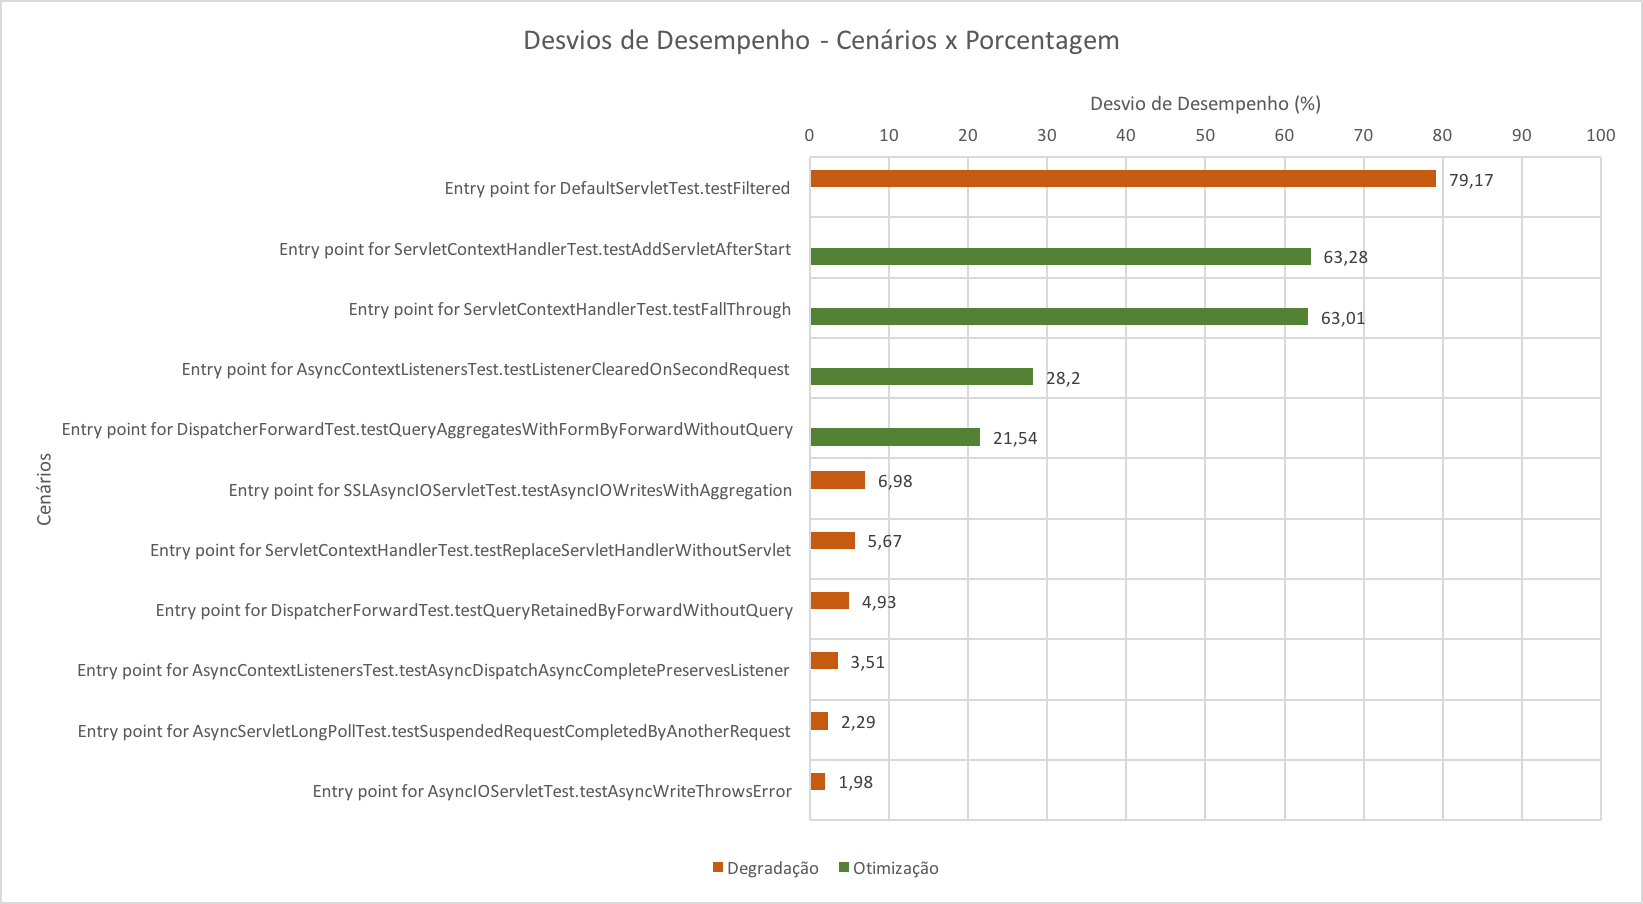
\includegraphics[scale=0.80]{Imagens/grafico_jetty_v926_v931M1.png}}
   \textsf{\caption[Porcentagem de desvios de desempenho para o Jetty, versões 9.2.6 para 9.3.0.M1.]{Porcentagem de desvios de desempenho para o Jetty, versões 9.2.6 para 9.3.0.M1.\label{fig:grafico-jetty-v9.2.6-v9.3.0.M1}}}
\end{sidewaysfigure}

\section{Considerações} \label{sec:consideracoes-cap3}


Um dos principais desafios do processo de manutenção de um software é compreendê-lo adequadamente, em especial, a sua arquitetura. A falta de acompanhamento da evolução da arquitetura ao longo do tempo pode levar a sua degradação, impactando os seus atributos de qualidade. Este capítulo apresentou visualizações de arquitetura de software que visam tornar direta e fácil a monitoração da evolução arquitetural, com relação ao atributo de qualidade de desempenho. Uma vez que as ferramentas existentes se mostram complexas ou ineficientes para essa finalidade, as visualizações foram propostas a serem implementadas como extensões da ferramenta \textit{PerfMiner}. Em suma, são as seguintes:
\begin{enumerate}[(i)]
   \item \textit{Evolução do Desempenho}: a evolução do atributo de qualidade de desempenho pode ser acompanhada em outra visualização, que mostra, para cada versão do sistema, se este degradou, otimizou ou manteve estável o seu desempenho;
   \item \textit{Sumarização dos Cenários}: a sumarização dos cenários com desvio de desempenho objetiva mostrar, de maneira sucinta, quais cenários analisados tiveram desvio de desempenho, seja degradação ou otimização;
   \item \textit{Grafo de Chamadas}: a visualização do grafo de chamadas exibe, para cada cenário, as chamadas dos métodos que tiveram desvio de desempenho. Dessa forma, o usuário pode localizar em qual trecho de código da execução do cenário houve o desvio.
\end{enumerate}

Foi mostrado os detalhes da visualização do grafo de chamadas, que visa exibir, para dadas duas versões de um sistema, os métodos que potencialmente causaram o desvio de desempenho para um determinado cenário. Nesta visualização, os métodos são apresentados em um grafo direcionado de chamadas com propriedades visuais que destacam quais dos métodos mostrados tiveram desvios de desempenho.

É importante frisar que a implementação das visualizações ainda não está finalizada. As duas primeiras mencionadas neste capítulo, evolução do desempenho e sumarização dos cenários, ainda estão em fase de concepção, ao passo que a terceira, grafo de chamadas, está em fase de conclusão. Para esta última, ainda serão adicionados, na seção de detalhes dos nós, \textit{links} para os \textit{commits} e tarefas que alteraram o método representado. Para cada método com desvio, serão recuperados os \textit{commits} do sistema de controle de versões e verificado quais commits alteraram linhas dentro do método detectado. Para cada um dos que alteraram, o número da respectiva tarefa é procurado na mensagem de \textit{commit}. Este número é usado para procurar a tarefa no sistema de gerenciamento de tarefas em busca de informações extras, como o seu tipo.

\section{Ameaças à validade} \label{sec:ameacas}
	
	% Capitulo 4: Quarto capítulo (arquivo Includes/Capitulo4.tex)
	% Capíulo 4
\chapter{Trabalhos Relacionados} \label{ch:trabalhos-relacionados}

	
	% Capitulo 5: Quinto capítulo (arquivo Includes/Capitulo5.tex)
	% Capíulo 5
\chapter{Trabalhos Relacionados} \label{ch:trabalhos-relacionados}

Este capítulo confronta este trabalho contra outras pesquisas que analisam a evolução do desempenho de sistemas. Qualquer trabalho ou ferramenta que mensure a evolução do atributo de qualidade de desempenho e possua visualizações para exibi-la é considerado relacionado a este. Na seção \ref{sec:trabalhos-relacionados-ferramentas-profiling} são comentadas as ferramentas de \textit{profiling}. Na seção \ref{sec:trabalhos-relacionados-ferramentas-apm} são mostradas as ferramentas APM. Por fim, na seção \ref{sec:trabalhos-relacionados-adordagens-degradacao-desempenho} são exibidas as abordadens de medição da degradação de desempenho.

Muitas abordagens relacionadas a visualização de software têm sido propostas para comparar versões de software de um ponto de vista geral da arquitetura \cite{Steinbruckner2010b}\cite{Telea2008}\cite{Collberg2003}\cite{Eick1992}\cite{Holten2008}. Outras abordagens focam em visualizar as métricas do software em diferentes versões \cite{Langelier2008}\cite{Lanza2001}\cite{Pinzger2005}\cite{Wettel2008}. No entanto, essas abordagens diferem deste trabalho uma vez que o objetivo é comparar um aspecto dinâmico do software, o desempenho, ao invés de aspectos estáticos ou estruturais.

\section{Ferramentas de Profiling} \label{sec:trabalhos-relacionados-ferramentas-profiling}

Há ferramentas de \textit{profiling} que podem realizar a medição do atributo de qualidade de desempenho, no entanto, com diferentes características. O \textit{JProfiler} \cite{JProfiler} e o \textit{YourKit Java Profiler} \cite{Profiler2016} são duas ferramentas comerciais para realizar profiling de aplicações na linguagem Java. \citeauthor{SandovalAlcocer2013} comentam algumas limitações dessas duas ferramentas:
\begin{itemize}
	\item \textit{Variações de desempenho têm que ser manualmente rastreadas}: para cada execução, o \textit{profiler} tem que ser manualmente configurado para executar uma versão em particular. Depois, os dados do \textit{profiling} podem ser salvos no sistema de arquivos. Após realizar esse procedimento por duas vezes, ambas as execuções podem ser comparadas. Entretanto, cada execução requer muito trabalho manual;
	\item \textit{Faltam métricas relevantes}: ambas as ferramentas não consideram se o código-fonte foi alterado ou não. Como consequência, variações de desempenho em métodos não modificados podem distrair o programador de identificar alterações de código que realmente introduziram as variações;
	\item \textit{Representações visuais ineficientes}: O \textit{JProfiler} e o \textit{YourKit Java Profiler} usam uma tabela textual incrementada com alguns ícones para indicar variações. Dessa forma, entender qual variação de desempenho decorre de mudanças de software requer um esforço significativo do programador.
\end{itemize}

Os autores comentam que essas ferramentas, apesar de serem úteis para acompanhar o desempenho geral, são ineficientes para saber a diferença dos tempos dos métodos e, muitas vezes, insuficientes para compreender as razões para a variação de desempenho. Há ainda uma ferramenta que acompanha a JVM, chamada \textit{VisualVM}, que possui as mesmas limitações comentadas anteriormente. Além disso, o \textit{VisualVM} não oferece a comparação entre execuções, tornando difícil a visualização da evolução do desempenho entre as versões do software, uma vez que teria que ser feita manualmente para cada método desejado.

\section{Ferramentas APM} \label{sec:trabalhos-relacionados-ferramentas-apm}

O trabalho de \citeauthor{Ahmed2016} realizou um estudo para verificar se as ferramentas de gerenciamento de desempenho de aplicações - APM - são eficazes na identificação de regressões de desempenho. Os autores definem regressão de desempenho quando as atualizações em um software provocam uma degradação no seu desempenho. As ferramentas utilizadas no estudo foram \textit{New Relic} \cite{Relic2016}, \textit{AppDynamics} \cite{Appdynamics}, \textit{Dynatrace} \cite{Dynatrace2016} e \textit{Pinpoint} \cite{Pinpoint2016}. Como resultado, eles mostram que a maioria das regressões inseridas no código-fonte foram detectadas pelas ferramentas. Contudo, o processo de identificação do método exato cujo código foi inserido foi mais complicado, sendo necessário bastante trabalho manual: os autores inspecionavam as transações (requisições) marcadas como lentas e, manualmente, comparavam os respectivos \textit{stacktraces} para verificar se a ferramenta indicava corretamente a regressão de desempenho.

A ferramenta e a extensão proposta neste trabalho é diferente das ferramentas apresentadas no trabalho de \citeauthor{Ahmed2016} por realizar a análise de duas versões do software alvo do estudo, por automatizar o processo de identificação da causa do desvio de desempenho, por prover visualizações adequadas à identificação dos desvios de desempenho, bem como exibindo dados adicionais dos nós do grafo, por mostrar a evolução global e por cenário do desempenho e por proporcionar aos desenvolvedores a identificação diretamente do código-fonte das causas do desvio de desempenho.

\section{Abordagens de Degradação de Desempenho} \label{sec:trabalhos-relacionados-adordagens-degradacao-desempenho}

O trabalho de \citeauthor{SandovalAlcocer2013} propõe uma abordagem visual para entender a causa de degradações de desempenho, comparando o desempenho de duas versões do sistema. Trata-se de uma visualização polimétrica, onde formas e cores dos elementos visuais indicam valores de métricas e propriedades do software analisado. O trabalho utiliza a ferramenta \textit{Rizel} para medição de propriedades dos métodos, tais quais: suas métricas, quais métodos foram adicionados, removidos ou modificados, e o seu tempo e número de execução. A abordagem foi desenvolvida na linguagem de programação Pharo.

O trabalho proposto se diferencia do de \citeauthor{SandovalAlcocer2013} pelo fato de: (i) ser compatível com a linguagem Java; (ii) exibir a evolução do desempenho global do software entre as versões; (iii) exibir a evolução de cada cenário entre as versões do softwares; e (iv) utilizar diferentes elementos visuais para destacar a evolução do desempenho na visualização do \textit{call graph} dos cenários.

\citeauthor{Bergel} propôs uma abordagem cujo objetivo é comparar duas versões de um software. A visualização exibe informações de execução como um \textit{call graph}, onde os nós são os métodos e as arestas são as invocações. Cada nó é renderizado como uma caixa e uma invocação é uma linha que une dois nós. No entanto, essa abordagem considera apenas se um método gastou ou não mais tempo de execução do que na versão anterior. O trabalho proposto se diferencia por adicionar mais métricas, como a porcentagem de desvio de desempenho dos métodos e se houve métodos adicionados ou removidos. Ainda, facilita a identificação da causa do desvio de desempenho, e irá prover aos desenvolvedores e arquitetos a possibilidade de verificar as mudanças no código-fonte ocorridas entre as duas versões comparadas.

\citeauthor{Mostafa2009} propõem uma técnica que compara duas árvores de contexto de chamadas \abrv[CCT -- \textit{Context Call Tree}]{}(CCT, do inglês \textit{Context Call Tree}), cada uma obtida de uma versão diferente de um software. Os autores apresentam o \textit{PARCS}, uma ferramenta de análise que identifica automaticamente diferenças entre o comportamento da execução de duas revisões de uma aplicação. Eles usam como base o algoritmo de correspondência de árvores comuns para comparar duas CCTs. No entanto, a abordagem, diferentemente deste trabalho, não detecta nenhum nó adicionado ou removido, o que é fundamental para o entendimento do real impacto de um novo nó no desempenho de determinada árvore de chamadas.
		
	% Bibliografia (arquivo Capitulos/Referencias.bib)
	\bibliography{Capitulos/Referencias}
	%\bibliography{Capitulos/library}
	\bibliographystyle{abnt-num}
	
	% Apêndice A (arquivo Includes/ApendiceA)
	% Apêndice
\apendice

\chapter{Informações adicionais sobre as aplicações analisadas }
\label{sec:apendice}

\section{Repositórios de código-fonte das aplicações}

\footnotesize
\begin{longtable}{| l | l | l |}
  	\hline
  	
  	% rótulo das colunas e infos de mudança de página
  	\textbf{Aplicação} & \textbf{Repositorio} & \textbf{Commit}  \\
 	\hline
 	\endfirsthead
 	
 	\multicolumn{3}{l}{\textit{Continuação da página anterior}} \\
 	\hline
 	
 	\textbf{Aplicação} & \textbf{Repositorio} & \textbf{Commit}  \\
 	\hline
 	\endhead
 	\hline \multicolumn{3}{r}{\textit{Continua na página seguinte}} \\
 	\endfoot
 	\hline
 	\endlastfoot
 	
 	%dados
 	AcDisplay		& https://github.com/AChep/AcDisplay 				 & 2ae3c79 \\ \hline
 	AFWall+			& https://github.com/ukanth/afwall 					 & 8c1f2d2 \\ \hline
 	aMetro			& https://github.com/RomanGolovanov/ametro 			 & a3f717a \\ \hline
 	AnkiDroid     	& https://github.com/ankidroid/Anki-Android			 & 1926fcc \\ \hline
 	AntennaPod  	& https://github.com/danieloeh/AntennaPod   		 & d5e63cb 	  \\ \hline
 	AnySoftKeyBoard & https://github.com/AnySoftKeyboard/AnySoftKeyboard & 7066bfe	  \\ \hline
 	\begin{tabular}[l]{@{}l@{}}
 			BatteryBot Battery \\ Indicator
 	\end{tabular} 	& https://github.com/darshan-/Battery-Indicator-Free & b20bb76	 \\ \hline 	
 	C:geo       	& https://github.com/cgeo/cgeo						 & 8fb79d3	  \\ \hline
 	ConnectBot		& https://github.com/connectbot/connectbot			 & cfafd40	 \\ \hline
 	Dash Clock		& https://github.com/romannurik/dashclock/			 & 8d9581d	\\ \hline
 	Document Viewer	& https://github.com/SufficientlySecure/document-viewer & 9fdef3d	 \\ \hline
 	\begin{tabular}[l]{@{}l@{}}
 	 	 	DuckDuckGo \\ Search \& Stories
 	\end{tabular}   & https://github.com/duckduckgo/android 	         & 87a605b	 \\ \hline
 	Firefox    		& http://hg.mozilla.org/mozilla-central				 & a66bf0a800f3	 \\ \hline
 	Focal (Beta)	& https://github.com/xplodwild/android\_packages\_apps\_Focal 	& d9cc873 \\ \hline
 	\begin{tabular}[l]{@{}l@{}}
 	     	 	 	Free Mobile \\Netstat
 	    \end{tabular} & https://github.com/vdavy/freemobilenetstat     & 118173d 	  \\ \hline
 	Google I/O   	& https://github.com/google/iosched	             	 & 2531cbd	  \\ \hline
 	\begin{tabular}[l]{@{}l@{}}
 	 	 		Hangar - Smart \\ app shortcuts
 	\end{tabular} 	& https://github.com/corcoran/Hangar 	 &	90c44705	\\ \hline
 	Indic Keyboard	& https://github.com/smc/Indic-Keyboard 			 & f52b974 \\ \hline
 	K-9 Mail      		& https://github.com/k9mail/k-9	                 & f794cc1	  \\ \hline
 	MyExpenses    		& https://github.com/mtotschnig/MyExpenses	     & ac08238	 \\ \hline
    \begin{tabular}[l]{@{}l@{}}
     	 	 	Numix Circle \\ icon pack
    \end{tabular} 		& https://github.com/numixproject/com.numix.icons\_circle 	& bdcf570	\\ \hline
    OpenTasks			& https://github.com/dmfs/opentasks 	         & b9e5d52	\\ \hline
 	\begin{tabular}[l]{@{}l@{}}
 	     	 	 	Orbot Proxy \\ com Tor
 	\end{tabular}	& https://gitweb.torproject.org/orbot.git 		 & 34079c7	\\ \hline
 	Persian Calendar	& https://github.com/ebraminio/DroidPersianCalendar & a4272cd	 \\ \hline
	Quick Dice Roller  	& https://github.com/Ohmnibus/quick-dice-roller 	& 32b2c1c	 \\ \hline
 	Ringdroid			& https://github.com/google/ringdroid/				& 81bdf25 	 \\ \hline
 	\begin{tabular}[l]{@{}l@{}}
 		Shattered Pixel \\ Dungeon
 	\end{tabular} 		& https://github.com/00-Evan/shattered-pixel-dungeon & aaadf4a 	  \\ \hline
 	\begin{tabular}[l]{@{}l@{}}
 		Simon Tatham's \\ Puzzles
 	\end{tabular} 	& https://github.com/chrisboyle/sgtpuzzles          & 6f170b5		   \\ \hline
    \begin{tabular}[l]{@{}l@{}}
    	Simple Last.fm \\ Scrobbler
    \end{tabular} 	& https://github.com/tgwizard/sls					& f7a3eca		\\ \hline
 	SnoopSnitch		& https://opensource.srlabs.de/projects/snoopsnitch & 4332a66		\\ \hline
 	Telegram 		& https://github.com/DrKLO/Telegram					& 2114024		\\ \hline
	\begin{tabular}[l]{@{}l@{}}
		Terminal Emulator \\ for Android
	\end{tabular} 	& https://github.com/jackpal/Android-Terminal-Emulator & f5ecc5a\\ \hline
 	Termux			& https://github.com/termux/termux-app 				& 746dc75	\\ \hline
 	Transdrone		& https://github.com/erickok/transdroid 			& 8b96074 	\\ \hline
 	Vanilla Music	& https://github.com/vanilla-music/vanilla 			& 94d6995	\\ \hline
 	VLC for Android & https://code.videolan.org/videolan/vlc-android 	& fad7ab3	\\ \hline
 	Vuze Remote     & https://github.com/vuze/vuze-remote-for-android 	& 118a52a	\\ \hline 			 	
 	\begin{tabular}[l]{@{}l@{}}
 	 	 		WiFiAnalyzer \\ (open-source)
 	\end{tabular} 	& https://github.com/VREMSoftwareDevelopment/WifiAnalyzer	& b9475a1 \\ \hline
 	Wififixer 		& https://github.com/Zanshinmu/Wifi-Fixer 			& 112da88		  \\ \hline
 	Yaac - IRC Client & https://github.com/pocmo/Yaaic 					& 5da4949		  \\ \hline
 	Zmanim        	& https://bitbucket.org/jgindin/zmanim				& 832:4ec02fb6be56\\ \hline
\end{longtable}


\section{IDs das aplicações na Google Play}

\footnotesize
\begin{longtable}{| l | l |}
  	\hline
  	
  	% rótulo das colunas e infos de mudança de página
  	\textbf{Aplicação} & \textbf{ID da aplicaçõe na Google Play}  \\
 	\hline
 	\endfirsthead
 	
 	\multicolumn{2}{l}{\textit{Continuação da página anterior}} \\
 	\hline
 	
 	\textbf{Aplicação} & \textbf{ID da aplicaçõe na Google Play}  \\
 	\hline
 	\endhead
 	\hline \multicolumn{2}{r}{\textit{Continua na página seguinte}} \\
 	\endfoot
 	\hline
 	\endlastfoot

 	%dados
 	AcDisplay		& com.achep.acdisplay \\ \hline
 	 	AFWall+			& dev.ukanth.ufirewall \\ \hline
 	 	aMetro			& org.ametro \\ \hline
 	 	AnkiDroid     	& com.ichi2.anki \\ \hline
 	 	AntennaPod  	& de.danoeh.antennapod 	  \\ \hline
 	 	AnySoftKeyBoard & com.menny.android.anysoftkeyboard	  \\ \hline
 	 	\begin{tabular}[l]{@{}l@{}}
 	 			BatteryBot Battery \\ Indicator
 	 	\end{tabular} 	& com.darshancomputing.BatteryIndicator	 \\ \hline 	
 	 	C:geo       	& cgeo.geocaching	  \\ \hline
 	 	ConnectBot		& org.connectbot	 \\ \hline
 	 	Dash Clock		& net.nurik.roman.dashclock	\\ \hline
 	 	Document Viewer	& org.sufficientlysecure.viewer	 \\ \hline
 	 	\begin{tabular}[l]{@{}l@{}}
 	 	 	 	DuckDuckGo \\ Search \& Stories
 	 	\end{tabular}   & com.duckduckgo.mobile.android	 \\ \hline
 	 	Firefox    		& org.mozilla.firefox	 \\ \hline
 	 	Focal (Beta)	& fr.xplod.focal \\ \hline
 	 	\begin{tabular}[l]{@{}l@{}}
 	 	     	 	 	Free Mobile \\Netstat
 	 	    \end{tabular} & org.pixmob.freemobile.netstat 	  \\ \hline
 	 	Google I/O   	& com.google.samples.apps.iosched	  \\ \hline
 	 	\begin{tabular}[l]{@{}l@{}}
 	 	 	 		Hangar - Smart \\ app shortcuts
 	 	\end{tabular} 	& ca.mimic.apphangar	\\ \hline
 	 	Indic Keyboard	& org.smc.inputmethod.indic \\ \hline
 	 	K-9 Mail      		& com.fsck.k9	  \\ \hline
 	 	MyExpenses    		& org.totschnig.myexpenses	 \\ \hline
 	    \begin{tabular}[l]{@{}l@{}}
 	     	 	 	Numix Circle \\ icon pack
 	    \end{tabular} 		& com.numix.icons\_circle	\\ \hline
 	    OpenTasks			& org.dmfs.tasks	\\ \hline
 	 	\begin{tabular}[l]{@{}l@{}}
 	 	     	 	 	Orbot Proxy \\ com Tor
 	 	\end{tabular}	& org.torproject.android	\\ \hline
 	 	Persian Calendar	& com.byagowi.persiancalendar	 \\ \hline
 		Quick Dice Roller  	& ohm.quickdice	 \\ \hline
 	 	Ringdroid			& com.ringdroid 	 \\ \hline
 	 	\begin{tabular}[l]{@{}l@{}}
 	 		Shattered Pixel \\ Dungeon
 	 	\end{tabular} 		& com.shatteredpixel.shatteredpixeldungeon 	  \\ \hline
 	 	\begin{tabular}[l]{@{}l@{}}
 	 		Simon Tatham's \\ Puzzles
 	 	\end{tabular} 	& name.boyle.chris.sgtpuzzles		   \\ \hline
 	    \begin{tabular}[l]{@{}l@{}}
 	    	Simple Last.fm \\ Scrobbler
 	    \end{tabular} 	& com.adam.aslfms		\\ \hline
 	 	SnoopSnitch		& de.srlabs.snoopsnitch		\\ \hline
 	 	Telegram 		& org.telegram.messenger		\\ \hline
 		\begin{tabular}[l]{@{}l@{}}
 			Terminal Emulator \\ for Android
 		\end{tabular} 	& jackpal.androidterm \\ \hline
 	 	Termux			& com.termux	\\ \hline
 	 	Transdrone		& org.transdroid.lite 	\\ \hline
 	 	Vanilla Music	& ch.blinkenlights.android.vanilla	\\ \hline
 	 	VLC for Android & org.videolan.vlc	\\ \hline
 	 	Vuze Remote     & com.vuze.android.remote	\\ \hline 			 	
 	 	\begin{tabular}[l]{@{}l@{}}
 	 	 	 		WiFiAnalyzer \\ (open-source)
 	 	\end{tabular} 	& com.vrem.wifianalyzer \\ \hline
 	 	Wififixer 		& org.wahtod.wififixer		  \\ \hline
 	 	Yaac - IRC Client & org.yaaic		  \\ \hline
 	 	Zmanim        	& com.gindin.zmanim.android \\ \hline
\end{longtable}

\section{Dados brutos}

Dados brutos obtidos durante o estudo podem ser acessados através da URL: http://bit.ly/multversion-android
	
	% Anexo A (arquivo Includes/AnexoA)
	%% Anexo
\anexo
\chapter{Primeiro anexo}

Os anexos são textos ou documentos não elaborado pelo autor, que servem de fundamentação, comprovação e ilustração.
	
	% Página em branco
	\newpage

\end{document}
